% !TEX encoding = UTF-8 Unicode
% !TEX TS-program = pdflatex

%%%%%%%%%%%%%%%%%%%%%%%%%%%%%%%%%%%%%%%%%%%%%%%%%%%%
%% TESI DI LAUREA MARTINA GHEDIN 
%% TOPIC MODA SOSTENIBILE
%%%%%%%%%%%%%%%%%%%%%%%%%%%%%%%%%%%%%%%%%%%%%%%%%%%%  Esempio con molte opzioni
\documentclass[%
    corpo=11pt,
    twoside, % impostazione per margini in libro
    %stile=classica,
    oldstyle,
    autoretitolo,
    greek,
    evenboxes,
%    tipotesi,
]{toptesi}
%%%%%%%%%%%%%%%%%%%%%%%%%%%%%%%%%%%%%%%%%%%%%%%%%%%%

\usepackage[utf8]{inputenc}   %% si può scegliere anche latin1, ma lo si sconsiglia 

\usepackage{comment}
\usepackage[T1]{fontenc}
\usepackage{lmodern}  
\usepackage{amsmath}            %% per la matematica estesa
\usepackage{lipsum}             %% Per scrivere testo fasullo in "latinorum"

%%\usepackage{natbib}
\usepackage{booktabs}           %% del Sistema Internazionale
\usepackage{latexsym}
\usepackage{caption}
\usepackage{subcaption}
\usepackage{graphicx}
\usepackage{listings}
\usepackage{color}
\usepackage{longtable}
\usepackage{wrapfig}
%\usepackage{longtable}
%\usepackage{setspace}
%\usepackage[margin=3cm]{geometry}
                                               
\usepackage{sidecap}   %% Didascalie a fianco della figura
\usepackage[autostyle,italian=guillemets]{csquotes}   %% Per il corretto funzionamento di BibLatex
\usepackage[sorting=none,style=numeric-comp,backend=biber]{biblatex}


% Vedere la documentazione italiana o inglese di TOPtesi
% per le attenzioni che bisogna usare al fine di ottenere
% un file veramente conforme alle norme per l'archiviabilità.


% Lasciare questo per ultimo dopo aver caricato tutti gli altri pacchetti
%
% Se si è già caricato hyperref anche indirettamente (tramite altri
% pacchetti) questo statement evita di ricaricarlo
\usepackage[a-1b]{pdfx} % è utile, tienilo
\unless\ifcsname ver@hyperref.sty\endcsname\usepackage{hyperref}\fi

\hypersetup{%
	pdfpagemode={UseOutlines},
	bookmarksopen,
	pdfstartview={FitH},
	colorlinks,
	linkcolor={black}, %pink
	citecolor={black}, %pink
	urlcolor={black}
}
%%%%%%%%%%%%%%%%%%%%%%%%%%%%%%%%%%%%%%%%%%%%%%%%%%%%%%%%%%%%%%%%%%%%%%%%%

%%%%%%% Definizioni locali
\newtheorem{osservazione}{Osservazione}% Standard LaTeX
\addbibresource{bibi2.bib}

\begin{document}
\english
%\onehalfspacing % Set line spacing to 1.5



\ateneo{\textsc{University of Trento}}
%\nomeateneo{Sede di Torre Elettra}
	\nomeateneo{Industrial engineering department}
	
	\titolo{Understanding the effect of opinions and behaviours on the spread of infectious diseases}
	%\sottotitolo{pensare ad un sottotilo}     
	\CorsoDiLaureaIn{Mechatronics Engineer}

\renewcommand*\IDlabel{\\\quad Student Id: }
	
 \candidato{Riccardo Tessarin}[222819]

	\relatore{Prof.~Giulia Giordano}
	
	\secondorelatore{Doct.~Daniele Proverbio}


	\sedutadilaurea{\textsc{Academic year} 2023-2024}
	\logosede[95 pt]{STN} %immagine del logo 
%%%%%%%%%%%%%%%%%%%%%%%%%%%%%%% Per mettere 4 relatori con classica
%\AdvisorName{Supervisors}% esempio per l'inglese
%\direttore{prof. Albert Einstein}% per il dottorato
%\coordinatore{prof. Albert Einstein}% per il dottorato
%    \relatore{prof.~Albert Einstein}% per la laurea e/o il dottorato
%    \secondorelatore{dipl.~ing.~Werner von Braun}
%    \terzorelatore{\tabular[t]{@{}l}
%    Mario Rossi\\[0.5ex]
%    Piero Negri
%    \endtabular}% per la laurea magistrale
%%%%%%%%%%%%%%%%%%%%%%%%%%%%%%% Alternativa senza opzione classica
%    \AdvisorName{Relatore}
%    \relatore{prof.~Giovanni Bianchi}
%    \secondorelatore{\tabular{@{}l}%
%    \bfseries Correlatori\\[0.5ex]
%    ing.~Lucio Verdi\\[0.5ex]
%    dott.~Mario Rossi\\[0.5ex]
%    dott.~Piero Neri
%    \endtabular}
%%%%%%%%%%%%%%%%%%%%%%%%%%%%%%% Alternativa con 4 relatori senza
%%%%%%%%%%%%%%%%%%%%%%%%%%%%%%% indicazione dei correlatori e senza
%%%%%%%%%%%%%%%%%%%%%%%%%%%%%%% opzione classica
%    \relatore{prof.~Giovanni Bianchi}
%    \secondorelatore{ing.~Lucio Verdi}
%    \terzorelatore{\tabular{@{}l}
%    dott.~Mario Rossi\\[0.5ex]
%    dott.~Piero Neri
%    \endtabular}

%%%%%%%%%%%%%%%%%%%%%%%%%%%%%%% Altro trucco per mettere il correlatore
%%%%%%%%%%%%%%%%%%%%%%%%%%%%%%% senza usare l'opzione classica
%\relatore{\tabular{@{}l@{}}
%prof.\ Albert Enstein\\[1.5ex]
%\textbf{Correlatore:}\\
%dipl.~ing.~Werner von Braun
%\endtabular}
%%%%%%%%%%
%
%%%%%%%%%% Trucco per scrivere anche un quarto relatore
%\terzorelatore{{\tabular{@{}l}dott.\ Neil Armstrong\\prof. Maria Rossi\endtabular}}

%%%%%%%%%%%%%%%%%%%%%%%%%%%%%%%%%%%%%%%%%
%%%%%%% Change the strings if you want a title page and a
%%%%%%% copyright page in another language
%%%%%%% Comment just the \iflanguage statement and the
%%%%%%% closing line of the language test if you want to
%%%%%%% make a global change instead of a conditional one.
%%%%%%% Comment the following indented lines if you don't
%%%%%%% care about the title page in English
\iflanguage{english}{%
	\retrofrontespizio{This work is subject to the Creative Commons Licence}
	\DottoratoIn{PhD Course in\space}
	\CorsoDiLaureaIn{Master degree course in\space}
	\NomeMonografia{Bachelor Degree Final Work}
	\TesiDiLaurea{Master Degree Thesis}
	\NomeDissertazione{PhD Dissertation}
	\InName{in}
	\CandidateName{Candidates}% or Candidate
	\AdvisorName{Supervisors}% or Supervisor
	\TutorName{Tutor}
	\NomeTutoreAziendale{Internship Tutor}
	\CycleName{cycle}
	\NomePrimoTomo{First volume}
	\NomeSecondoTomo{Second Volume}
	\NomeTerzoTomo{Third Volume}
	\NomeQuartoTomo{Fourth Volume}
	\logosede{STN}% or comma separated list of logos
}{}


%\ifbool{classica}%

  

\frontespizio % sarebbe meglio usare l'ambiente


\begin{dedica}
	To my old friend Gojira
	
\end{dedica}
\paginavuota
\sommario 

Slow fashion is a movement born recently to contrast the fast fashion trend. It consists in implementing a better and more sustainable supply chain with a positive environmental and social impact. Nevertheless, there is a common bias where people perceive ethical products to be too expensive. This is due partially to the actual high prices of some brands but it is also a consequence of greenwashing. In order to investigate this aspect, an empirical research has been conducted with Atotus.
It is both an e-commerce and a physical shop in Trento that sells ethical articles of clothing as a core business and it has built a circular economy network. 

A choice based conjoint analysis is performed. The first step is to build two different surveys, which have been submitted to individuals through two channels. Both questionnaires present three product profiles and individuals choose the one they would buy. Each profile is composed by one level of each attribute. These attributes are design, material and price.

Respondents are actual and potential Atotus customers reached through its social networks. Next, the collected data are given as input to the multinomial logit model to identify respondents preferences across attributes. It is the standard model, where only the individual-specific variables are taken into account. The advanced or mixed multinomial logit model includes more detailed aspects, such as heteroscedasticity and random parameters. Moreover, the willingness to pay (WTP) and the market shares of sustainable products are investigated. 

The analysis shows that all attributes are equally significant for respondents. This is the case both for the standard model and the mixed one. Moreover, the WTP shows that respondents would pay €38 more in order to buy a t-shirt made of recycled cotton and €34 for a t-shirt made of certified organic cotton. Additionally, the design, p1 and p2 are the preferred ones. As regard the shares prediction, almost 50\% of individuals would buy a product made of a  sustainable material of design p1 or p2 with a price of 50€. 

There is not much literature regarding this specific topic. Indeed, conjoint analysis is performed in many fields, but slow fashion has not been one of them. These results show a starting point of applied data analysis in this specific field. Additionally, it is possible to notice that there is a strong interest among potential and actual customers toward Atotus products and individuals' purchase behavior is coherent with Atotus pricing strategy.

%%%%%%%%%%%%%%%%%%%%%%%%%%%%%%%%%%%%%%%%%%%%%%%%%%%%%%%%%%%%%%%%%%%%%%%%%%%%%%%%%%%%

% \paginavuota 


  \tablespagetrue     %% Lista delle Tabelle
  \figurespagetrue   %% Lista delle Figure
  \indici	             %% Produce l'indice




%%%%%%%%%%%%%%%%%%%%%%%%%%%%%%%%%%%%%%%%%%%%%%%%%%%%%%%%%%%%%%%%%%%%%%%%%%%%%%%%%%%%%%%%%%%%%%%%%%%%%%%
%%% Qui Inizia il corpo dell'elaborato vero e proprio
%%%%%%%%%%%%%%%%%%%%%%%%%%%%%%%%%%%%%%%%%%%%%%%%%%%%%%%%%%%%%%%%%%%%%%%%%%%%%%%%%%%%%%%%%%%%%%%%%%%%%%%
%\mainmatter]


\part{Introduction}

\chapter{Introduction}

What has been one of the main dangers humanity has faced throughout its history? The first answers that can be given are war or climate change, but there is another great threat that has severely affected the lives of almost all the population on earth: disease and epidemic. There is not a period neither nowadays nor in the past in which illness has not influenced our lives. 

Looking to the past the consequences of the epidemic on the population were worse than today because of the lack of knowledge about medical science and the poor hygienic conditions.  During the bubonic plague of the 14th century, for example, 25 million deaths were reported in Europe out of a population of 100 million. Jews were considered responsible for the illness spread and they began to be persecuted.
Otherwise, in the course of the Americas' colonization, the disease imported by the Europeans was one of the main causes of the genocide of the local population, causing their defeat against the Spanish conquistadores. In fact, diseases like smallpox and cholera were unknown in these countries and native Americans had no antibodies to contrast them. 
Other important epidemics, famous for their consequences were Spanish influenza, Smallpox, Typhus, HIV/AIDS, and the more recent Covid-19. 
It is straightforward to notice the effect that diseases have on our lives.

The development of modern medicine and hygiene can contribute to enhancing the quality of life. An example of this is that only in the last three centuries and especially in the most economical developing countries, a significant increase in life expectancy has been observed \cite{Anderson_82}.
%riscrivi meglio ma intanto ci sta. 
This increase is also happening in the poorest region, like Subsaharian Africa, and even if actually their life expctancy value is lower, newest research predict that they will have the gratest increase in the next thirty years \cite{Vollset_2024}. This study also predict that the phenomena will cause a convergence in the life expectancy between now and 2050.  

perchè succede:
"Across locations, the burden of disease will continue to shift from communicable, maternal, neonatal, and nutritional
diseases to non-communicable diseases." 
questa è la chiave e lo stesso articolo dice che  è dovuto a una diffusione sempre più permeante della sanita e di norme coadiuvate a livello di macro r egione per gestione di malattie e che questo trend va mantenuto. 
ALLEGA ANCHE LA FIGURA PRESA DALL'ARTICOLO A STO PUNTO. 

 Even if mortality is decreased, the modification in social patterns and the development of large cities, have had some consequences: a higher density of population has increased in the $18^{th}$ and $19^{th}$ centuries the frequency and magnitude of epidemics.
\begin{figure}[h]
	\centering
	\includegraphics[width=0.85\linewidth]{0_introduction/images_introduction/worst_epidemic}
	\caption[Epidemic distribution in time]{A graphical representation of the epidemic distribution over the years and of their associated death toll. It is observable how there are an increment in the number of these event in the last three century.}
	\label{fig:worstepidemic}
\end{figure}


  As it can be seen in \ref{fig:worstepidemic}, even if some improvements in health status were achieved, the presence of new disease potentially escalating in an outbreak is a concrete menace that needs attention and consideration on health policies. 

However, the health status is not the only aspect concerned with a disease. Being sick causes profound modification in our relationship, work, and social life, for example, causing a deterioration of also the social health. 
There is also an economic cost associated with the cure necessary to be healed. Only in a few nations worldwide, is treatment covered free of charge by the state. In the majority, being ill can result in having to sustain high costs, causing people to go into debt or not take care. 
All these effects sum together and influence how populations behave when facing an epidemic. What are the consequences of adopting a certain behavior during a disease outbreak? It's a crucial question and can help to understand how to develop more efficient policies for contrasting epidemics. It is also the question that represents the first objective of study for the present work: can a multidisciplinary-based model be developed, integrating social and epidemiological features and analyzing their mutual relationship during a disease spread? 

Taking a step back, it's important to understand why epidemic models are crucial and what this field of research entails.
When a new disease emerges, the primary objective is to develop a defense against it. This begins with an epidemiological investigation to understand the disease's origin, the biological mechanisms behind its spread, and its resistance to existing drugs. The goal of this investigation is to gather all available information and understand the unfolding situation.
The next critical step is to study the disease's dynamics and create a model to predict its evolution. This requires understanding and estimating various parameters related to the disease. Key factors include the transmission mechanism within the population, the reproductive rate of the infectious agent in the host, the acquisition and persistence of immunity, and the contagion mechanism.
Developing a reliable model is scientifically valuable and serves as a powerful tool for stakeholders. It helps in formulating the best policies to implement during a pandemic emergency. For this purpose, theoretical epidemiology must adapt to provide insights and policy advice. Data acquisition and analysis are fundamental for statistically modeling epidemic coefficients. It is crucial to verify theoretical models against real-world data, as unverified theories cannot be validated.
In the end, a model capable of answering stakeholders' questions and making predictions, with or without the implementation of safety regulations, has numerous effects and outcomes on society. It is important to remember that, beyond the economic costs associated with every illness, there are also social costs. Developing instruments to better understand the spread of a disease can help mitigate its impact and lessen the social burden on society also preventing the loss of many lives.

\begin{figure}[]
	\centering
	\includegraphics[width=0.4\linewidth]{0_introduction/images_introduction/FlorentineCodex_smallpox}
	\caption[smallpox on native Americans]{Representation of smallpox disease on the Mexican population in the $XIV$ century. Figure from the Florentine Codex \cite{Sahagun1965}. }
	\label{fig:florentinecodexsmallpox}
\end{figure}
A first straightforward example, of the possible beneficial effects of having an epidemic model, is the possibility of arriving at the synthesis of "simple" parameters, specific for the disease under study, that can respond to questions like:
\begin{itemize}
	\item is this disease so infective that can cause a pandemic?
	\item what are the threshold conditions that can cause an outbreak? 
\end{itemize}

At first glance, the problem may appear straightforward. However, the creation of a model capable of evaluating every disease remains an unsolved challenge. Research in this field necessitates a careful balance between simplification and maintaining accuracy.

Over the past century, various aspects of epidemics have been extensively studied. Notable achievements by scientists include:
\begin{itemize}
	\item Development of epidemiological models using different mathematical tools, such as differential equations and agent-based networks.
	\item Predictions about the progression of epidemics or reconstructions of the events' dynamics.
	\item Insights into epidemics, explaining phenomena like the periodicity of re-infection for certain diseases or the seasonal patterns observed in cases such as influenza.
	\item Understanding the effectiveness of specific strategies against outbreaks, such as vaccines.
\end{itemize}
Furthermore, by using multilayer networks or systems, more complex analyses can be performed. The objective is to create models capable of simulating the evolution of multiple phenomena simultaneously or to develop a more accurate representation of the real world by constructing more intricate scenarios. Examples of such models include:
\begin{itemize}
	\item The simultaneous evolution of two different diseases.
	\item The formation of public opinions during an outbreak.
	\item The progression of a disease for which a vaccine exists, but where there is public fear of both the disease and potential vaccine side effects.
\end{itemize}
The work presented in this thesis is part of this type of research. A new model has been developed based on a study of existing multi-system models that integrate epidemic and behavioral or opinion components. Specifically, it is considered interesting to simulate a scenario in which the population is divided into three groups: those who have a positive opinion about the use of safety procedures and follow rules to avoid the transmission of the disease; a second group that opposes following procedures or recommendations, refusing to modify their behavior; and a third group that lacks information about the epidemic situation. This third condition represents the majority of the population when a new disease emerges, as there is limited information available and not yet widely disseminated.
In the model, the main mechanism used to change behavior among different social groups is peer pressure. The fatigue from belonging to a certain behavioral spectrum (either being compliant with the rules or against them) is also considered. An epidemiological model capable of tracking both the initial phase of an epidemic and successive waves of contagion is developed, including the possibility of reinfection.
A last feature of the work is the verification of its prediction with the use of real data. It is important for a novel multi-system model like the one implemented to have a comparison with reality. When two separate models are coupled together the result is not simply the sum of their previous characteristics, but other different phenomena can arise. Having a study, like the one performed by Meta during the Covid-19 pandemic about people's behavior is an incredible source of data that can permit us to interpret correctly the results given by the model. 
For this reason, the model's ability to reproduce what happened during the pandemic was initially tested. Then it was verified whether the peer pressure effect alone was sufficient to obtain the observed trends in population behavior or whether the addition of an external, global control factor, such as that represented by special laws implemented by governments, was necessary.

The main result achieved is that the model is functional and demonstrates reliability when compared with COVID-19 data. The study highlights the crucial importance of respecting quarantine measures and avoiding contact when infected, as these actions can significantly reduce the model's reproduction number, thereby limiting the spread of the disease. Altri risultati arriveranno concludendo la tesi.

\chapter{Main objectives and summary of the contents}

In this chapter, the main objectives pursued with the current work are presented and it is described the composition of the thesis. 
Starting from an analysis of the theoretical contributions already developed for epidemiology, and in particular focusing on multilayer systems and mean-field models, the following questions are studied:

\begin{itemize}
	\item how can be modeled in an effective way population behavior? What are the characteristics that must be considered?
	\item Can people's behavior influence the development of an epidemic?
	\item Is it sufficient to stop an outbreak by relying on the natural subdivision of the population into compliant and non-compliant groups regarding safety measures, or is the intervention of a central "controller" necessary to set new behavior rules?
	\item What is the most efficient way to model population collective consciousness about the epidemic's development? 
\end{itemize}
About the last question, consciousness or awareness is a parameter considered useful to gain insight into society's reaction to the disease. Furthermore, there can be differences in behavior when the same conditions occur at different times, such as at the beginning of an outbreak versus several months later. The quantity and quality of information available to the population can make a difference in how deal with difficult situations.

Starting from these questions, the following objectives have been identified:
\begin{itemize}
	\item Create an original epidemic-behavioral multi-system model capable of tracking the development of a disease and representing behavior modification using a peer pressure mechanism within the same population.
	\item Add a second control agent to the model, represented by government rules that can modify people's behavior in a centralized way.
	\item Develop a comprehensive analysis of the epidemiological and behavioral model to understand its mechanisms and correctly interpret the mutual effects arising from the coupling of the social and health systems.
	\item Conduct a study using available data on population behavior during the COVID-19 pandemic to verify if the developed model can accurately reconstruct events and how people reacted to them.
\end{itemize}
The work consists of an introductory chapter where the main concepts of social science and epidemiology are presented. This chapter provides all the necessary information to understand the research. It includes a glossary of the most important terms and an overview of the mathematical tools used in epidemiology. Additionally, the different models implemented to simulate an epidemic are shown, with a focus on the properties of the mean fields model, which is the primary model used in the thesis. Furthermore, a historical background of the research field is provided to give a perspective on the principal milestones.
In the third chapter, a review of the literature analyzed for the thesis is presented. The articles are categorized into different main topics: epidemiology theories, opinion models, behavior models, and multi-agent and multi-system models. This subdivision highlights the most interesting aspects of each work and identifies the elements that have been considered for inclusion in the thesis.
The second part of the thesis is composed of three main chapters. In Chapter Four, the chosen epidemiological and behavioral models are simulated, and their characteristics are studied individually. Chapter Five presents the model resulting from the integration of the two, which becomes a layer of a more complex multi-system model. The main features of this model are analyzed using analytical tools. The study is performed with theoretical values, sensitivity analysis, and the measurement of principal metrics, such as the reproduction rate, to provide a general description of the model and develop an understanding of it.
In Chapter Six, the data analysis is presented. The data available from the Meta COVID-19 research are used to test and validate the model, assessing its ability to represent a real scenario. Finally, the last chapter contains the conclusions of the thesis.
 

% ! Ci sta inizialmente concentrarsi sulle epidemie, ma  devi intrudurre anche il secondo macro filone, quello delle opinioni. é uno spin off metodologico del primo, quindi gli stumenti matematici poi sono simili, ma va detta anche questa cosa. E poi sulle opinioni hai visto quante sfumature diverse esistono sul come considerarle e anche questo è da tenere in considerazione. 
\chapter{Theoretical background}

\section{Epidemiological theory foundations}

Having a clear description of the main concepts in social science and epidemiology is essential for understanding the rest of the work developed. In the first section of the introduction, the theoretical basis and main concepts that will be used in the present work are defined. First, a brief historical review of the milestones in the field of epidemiology is provided, followed by a glossary of the main terms used in this thesis. Finally, the most commonly used mathematical tools are presented.
\subsection{ Epidemiologic research historical background}
% Se ti piace l'idea di fare un piccolo excursus storico, va bene. Le info principali sono:
% 1- primo lavoro di Bernoulli
% 2- lavori di Hamer (1906) mass action principle, epidemic description in discrete time 
% 3- Ross, formulation in continous time 
% 4- Kermack and Mc Kendrick (1927) che danno risultato bello perchè introducono "legge" del thresold di una epidemia
% Dopo aver scritto quest'ultimo evento hai il LA per parlare di come funziona un mean field model. 

The research field regarding the development of technique to understand how epidemics can evolve during time has a history starting back in the 20th century. The first important discovery in this field must be attributed to the scientists that find the mechanism used by disease to spread. 
A first innovative work is the one done by John Snow, that during an epidemic of Cholera in London in 1854 successfully determined the source of the infection, even without knowing its etiological agent. Then advancing in the microbiological research is conducted by Pasteur and Koch. They found the etiological agent of disease, enabling the possibility to treat and prevent people from an infection. 
Then, Hamer work in 1906 added a first major theoretical contribution. He formulated a theory about the correlation between the course of an epidemic and the interaction, contact ratio, between susceptible and infectious individuals. It is the so called “mass -action” principle. The number of contacts between these two groups determines the spread rate of the disease. 
This law originally written in discrete time, is then updated in 1908 by Ross, that re-written it  in continuous time. For the first time the problem can be studied using a clearly, well defined mathematical theory. Then the contributions of Kermack and McKendrick in 1927 add another fundamental principle to the modern epidemiology. They formulated a threshold theory explaining which condition can generate the development of an epidemic. The theorem affirms that a certain value must be exceed, depending on the proportion of susceptible and infectious individual. Controlling this value permits to understand if the number of infections will increase, until a peak is reached or if the epidemic is a descendent phase \cite{Mata2021}, \cite{Anderson_82}. 
Their contribution with the mass action principle represents the base for the mean field model theory, that will be presented and analysed in section \ref{subsec:SIR}. 



\subsection{Epidemiological glossary}
To permit a better comprehension of the subject analyzed in the present work a list of principal concepts and terms is presented.

\subsubsection{Micro and Macro parasite}
	The first difference when presenting infection is distinguishing the type of origin that can cause it. An etiological organism responsible for a disease can be divided into microparasite and macroparasite. The former live and reproduce within the host, generating an immune response and the infections caused by them usually have two possible outcomes: death or immunity. Infections origins from them are shorter than the life span of an individual, and so have a transient nature.
\subsubsection{Types of infectious diseases}
Infectious disease is indicated as an illness resulting from the presence of a pathogenic microbial agent. It is possible to distinguish a difference between \textit{transmittable} and \textit{communicable} disease. A transmittable disease can transmitted between persons through unnatural forces. A disease is communicable when the transmission happens directly or indirectly.

\subsubsection{Disease transmission} A disease can spread in different ways: 
	\begin{itemize}
		\item person to person, for example sexual transmission, involving direct or indirect contact.
		\item airborne, through inhalation of infected air.
		\item food or water borne, ingesting contaminated food. 
		\item vector born, the contagion is caused by infected animals.
	\end{itemize}
	Furthermore when the diffusion is among the same generations is called horizontal transmission, while vertical transmission is the one developing between different generations, from parents to children. 
	Zoonosis is the phenomenon in which a disease that starts in an animal species mutates and attacks humans. The opposite can also happen and it is called inverse-zoonosis. 
	
\subsubsection{Epidemic disease} It occurs when there is a disease with a rapid outbreak, in less than a year there is its development and a peak is reached. The illness is confined to a limited region

\subsubsection{Endemic disease} It is a disease that lasts for a long time and requires consideration of its impact on population renewal and in the number of susceptible individuals.

\subsubsection{Pandemic disease} It is an epidemic that diffuses across multiple regions, on a global scale. The severity of the disease also makes a distinction in calling a disease a pandemic. For example, a common cold is diffused in the whole world but is not defined as a pandemic by the WHO (World Health Organization). 

\subsubsection{Incubation, Symptoms, Infected and Infectious}   A person having contact with another infectious individual, can or not become infected. The incubation is the period after being infected in which the infection increases in size or number in the host but does not produce the symptoms, that are the effect of the disease. 

\subsubsection{Outbreak} Is the rapid raise in the number of infected during an epidemic.

\subsubsection{Incidence and prevalence} The first term refers to the number of new cases after a certain period (daily or weekly for example), while prevalence is the proportion of the population affected by a disease in a specific time.

\subsubsection{Immunity and herd immunity} Immunity is protection from a disease gained after having contracted it. It can last forever or vanish after a certain time. New exposure to the virus does not lead to infection. Herd immunity is instead an important phenomenon in which the defense against a disease is due to the majority of the population being immune, thanks to vaccines or surviving it. This majority protects the rest of the population because slows down the diffusion or stops the spread of the illness.

\subsubsection{Virulence and Contagiousness}  Virulence is used to describe how aggressive, harmful, and pathogenic is a biological agent in attacking cells. Contagiousness is referred to an individual and it is used to represent the capability to transmit a disease. 

\subsubsection{Overdispersion and Superspreading} Overdispersion is a term that refers to observing a larger variance than expected from a normal distribution. It is used in statistics to measure superspreading, a circumstance in which there is an anomaly (higher) number of secondary infections.

\subsubsection{CFR, IFR and mortality excess} The case fatality rate is the ratio between the number of deaths due to a specific disease and the total number of confirmed positive cases. It is the likelihood for an infected person to die because of the infection. The infection fatality rate is instead the percentage of people infected with the disease that are expected to die. The two quantities can have a similar value: if every person who contracts the disease and every death attributable to the disease is known and recorded, then the CFR will equal the IFR.
The excess in mortality can be calculated by observing the difference between the total death rate (due to any reason) a month per month in a comparison between a year with an epidemic and one without. 

\subsubsection{Reproduction number $R_0$} It is the fundamental measure of the infectiousness of a disease. It is the average number of secondary infections caused by one infected person in a fully susceptible population. If it is recalculated during the epidemic progression is called $R(t)$, a time-varying reproduction number. Finally exist also the effective reproduction number, describes the average number of secondary infected people during the epidemic (rescaling the value with the true number of susceptible). 


\subsubsection{Incubation period and serial interval} The incubation is the time after exposure in which the disease develops and ends when the infected start to show symptoms. The serial interval is instead the time that exists between two transmissions in a chain of infections. 

%%%%%%%%%%%%%%%%%%%%
\section{Opinion/behaviour glossary}
To establish a framework suitable for developing and understanding behavioral models, the following key concepts from social science are outlined.
\subsubsection{Awareness} It is the knowledge that an individual has on a certain subject or situation. It changes with time and it is developed with information or experience.  
\subsubsection{Information} The term "information" is often understood as "knowledge communicated." However, due to its central role in contemporary society, there is extensive debate regarding its multiple meanings \cite{Capurro_2003}. Our society can be characterized as an "information society," where the development of information technology has influenced all aspects of life. Currently, the word "information" is associated with two principal meanings. The first, more universal definition, is that information is anything important in answering a question. The second relates to Information Science, the discipline focused on managing this object called information in any form.
\subsubsection{Belief} It is the conviction of the truth of a statement or the reality of a being or phenomenon, especially when based on the examination of evidence, but also on matters for which there is no proof.

Studying beliefs change over time and on social networks is an interesting research field. It has the aim to understand why in certain societies new beliefs - such as opinions on climate change or anti-vaccinism spread more quickly than in others. These dynamics can lead to polarization or consensus and occasionally cause backlash effects.

\subsubsection{Behaviour} It is how one acts or conducts oneself. It can depend on the response of external stimuli and have effects, especially on others.
\subsubsection{Trust} It is the sentiment of confidence associated with the ability, strength, and truth of someone or something. 

\subsubsection{Perception} It is the mechanism for which something is regarded, understood, or interpreted.

\subsubsection{Group decision-making} It is a phenomenon at the intersection of psychology, management, biology, and applied mathematics studying how people in groups interact, exchange information, and realize decisions. The decision made by the group is no longer attributable to any single individual but to the whole group. 
 
\subsubsection{Threshold theory}

It is a theory formulated by Granovetter in \cite{Granovetter_1978} regarding collective behavior. The theory posits that in a society where individuals face two possible alternatives, and their choices involve certain costs and benefits depending on how many others choose each alternative, an individual will decide based on the number of others who have already chosen a particular option when this number exceeds a certain threshold.

\subsubsection{Polarization and Consensus}

Polarization refers to the variation in beliefs within a population.There are multiple meanings that can be associated to this term. One way to describe it is by measuring the distance between the most extreme beliefs, their spread or at the distribution of opinions in a certain interval. 

 The use of groups, identifying different concentration can be useful to explain the polarization phenomenon. Groups can be "exogenously" defined where are identified by characterstic like regionality, ethnicity, sex, education level, or other cathegories. To describe correctly the polarization a clear definition of the groups in consideration is necessary. 
 A first polarization group based is community fracturing, where the population is divided into subgroups\cite{Bramson_2017} .
 
 This contrasts with the term "consensus," which describes a situation where the exchange of opinions, information, or property among individuals leads to general agreement. Both scenarios are studied and modeled using network theory.

\subsubsection{Homophily} The tendency to bond and associate with similar others. 

\section{Epidemiological models categorization}
Starting from the observation of the real world, the desire to understand better a certain phenomenon is the fundament of mathematical model development. A perfect model does not exist, because it is based on data or on assumptions that are incomplete w.r.t reality. However, a useful model guarantees the possibility of realizing general predictions and can be a powerful instrument for policymakers.  For example, an application is the estimation of certain policies' effects on the population during an epidemic. So, the aim is to have meaningful results, under a given set of real-world circumstances.
When working on a model the importance of the uncertainty related to claims realized with this instrument must always remembered. This concept is remarked also on the definition of mathematical model present in \cite{Ledder_2023}. 
\begin{displayquote}
	"A Mathematical model is a self-contained collection of one or more variables together with a set of rules (usually formulas and equations) that prescribe the values of those variables. Models serve as an approximate quantitative description of some actual or hypothetical real-world scenario. They are created in the hope that the behavior they predict will capture enough of the features of that scenario to be useful."
\end{displayquote}

There are several different typologies of mathematical models developed.
A first classification can be done considering the method used to obtain them: mechanistic, empirical, or conceptual models.
The mechanistic model is based on assumptions about reality, or theoretical principles, modeled using a collection of one or more variables together with a self-contained set of rules. These models have an explanatory value on the reality they represent.
Empirical models are realized by fitting a set of data. It is a powerful instrument, because data can be modeled quite well, but they lack the explanatory value of the mechanistic model.  Finally, with conceptual model, it is meant a verbal description of a real-world scenario. 

For the present work, the mechanistic model is the strategy used.  This is because, in the epidemiology field, the scopes that conduce to the realization of a model go beyond just fitting data. Examples of possible scopes are:
\begin{itemize}
	\item following the epidemic evolution
	\item collect and realize a structure to understand the information related to the disease 
	\item obtaining general insight about control strategies
	\item realize predictions
\end{itemize}
Considering the mechanistic category several different types of models have been developed or are adapted to be used in epidemiology modeling. In this section, the principal typologies are now introduced. 

 There is then a focus, in \ref{subsec:SIR}, because it represents the mathematical base model of the multi-layer system implemented in the present work. It is important to introduce the logic underlying its structure, its main mechanisms, and the first important conclusion that can be derived from it because it is a useful introduction to the approach that will later be employed in the rest of the thesis.

\subsection{Mean field models}
\label{subsec:mean_field}
The mean field model, also known as compartmental model is the first developed and most studied type of mathematical model used in epidemiology \cite{kermack1927}, \cite{brauer2012mathematical}, \cite{Anderson_82}, and \cite{anderson1991infectious}.  This model assumes that the well-mixed population is divided into several subgroups. Each compartment is a different stage of the disease under consideration. Some possible states are susceptibles, asymptomatic (infected), symptomatic (infected), infected, exposed, vaccinated, quarantined, dead, recovered, and hospitalized. The classes considered in the realized model determine is base structure. The choice to include a certain compartment depends on the disease that is modeled and on the assumptions that are under analysis. Different models can be suitable to analyze the same disease but can be used with different aims. The difference is that a more complex model can emphasize some aspects or effects of the disease, that are not highlighted by a simpler one. 
In this class of model, the severity of infection usually is not considered: people are infected or not. The transition from one compartment to another is determined by differential equations. There are parameters ruling the transition between groups that are coefficients whose meaning depends on the model's underlying assumptions. The most important metric in this class of models is the so-called "basic reproduction number". It expresses the seriousness of a disease and it is considered the fundamental threshold in epidemiology \cite{Hernandez_Vargas_2022}. 
\begin{figure}[]
	\centering
	\includegraphics[width=0.65\linewidth]{0_introduction/images_introduction/SIRS_figure_compartmental}
	\caption[SIRS example]{An example of the graph structure of a mean field SIRS model. There are three compartments and the flow rate between them is ruled by the coefficients $\beta$, $\gamma$ and $\delta$.}
	\label{fig:sirsfigurecompartmental}
\end{figure}


\subsubsection{SIR model}
\label{subsec:SIR}
The model that represents the base for epidemic mathematical studying is the SIR.  Here the population or density of individuals is divided into three groups: Susceptible, Infectious, and Recovered. At time $t$ the three groups are identified with the symbols: $S(t)$, $I(t)$, and $R(t)$. 
The symbols used to indicate the density of each group are $s$, $i$, and $r$, while the capital letters are used to specify both the name of the groups or the absolute number of participants in each one. 
Usually, the assumption that N remains stable is made. This is possible considering that the term epidemic identifies a disease with a duration much lower than the life of a person. Considering this assumption the number of deaths and births can be neglected. Alternatively, we can consider that the number of births, which is an influx in the S compartment is roughly equal to the number of deaths, which is an outflux. These statements imply $s(t) + i(t) + r(t)= 1$ and $\dot{s}+ \dot{i} + \dot{r}= 0$.
The disease reproduces horizontal incidence within the population. So, it is the connection with others that causes the infection diffusion. 
$\beta$ is a coefficient that expresses the number of adequate contacts on average of a person per unit of time. The simplest way to explain the meaning of $\beta$ is to consider that not every contact between a susceptible and an infected person can generate a contagion. The formula  $\beta \frac{I}{N} = \beta i$ is then the average number of contacts with infectives per unit time of one susceptible. Finally, the number of new cases per unit of time due to the $S = N s$  susceptibles is $\beta \frac{I}{N} S = \beta N i s$. This form of horizontal incidence is called the standard
incidence. In this incidence, there is no dependence on population size \cite{Hethcote_2000}. This is because the contact of individuals daily is independent of the country dimension in which they live. 

The second transition process in the model is that individuals move from the infectious state to the recovered one at a rate $\gamma$. So the infection duration lasts an average time of $1/\gamma$ days. The $\gamma$ parameter represents the healing or recovery rate of the population. A mathematical interpretation of this term is that  
corresponds to exponentially distributed waiting times in the $I$ compartments. The transfer rate $\gamma I$ corresponds to $P(t) = e^{\gamma t}$. It is the fraction of infected that are still in their class after time $t$ of entering it and with a mean waiting time of $\frac{1}{\gamma}$.


%%
In this initial model, the immunity acquired after recovering from the illness is lifelong. It is equivalent if after being sick a person recovers or dies because it is considered that it will not transmit the infection anymore.  This assumption can be modified and there are often diseases in which after a certain period individuals become again susceptible. Another initial simplification is the one of considers the coefficient $\beta$ and $\gamma$ constant. 

Although the SIR model is quite simple it can predict a very important aspect of an epidemic, the threshold value. This effect was the main novelty studied in the pioneering work of Kermack and McKendrick \cite{kermack1927}. They found that in a fully susceptible population if and only if R0 > 1 an infection can start diffusing. Thus the origin of the term "threshold value" in epidemiology. 

The dynamic of this system has been extensively studied and analyzed during the years \cite{Breda_2012}, \cite{akinboro2014numerical}, \cite{Jard_n_Kojakhmetov_2021}, \cite{Ledder_2023}, \cite{Okabe_2020}, \cite{Prodanov_2022}, \cite{Xu_2014}, and \cite{Turkyilmazoglu_2021}. The threshold effect distinguishes between two scenarios. The first is when $R_0 <1 $. It is called "free disease equilibrium. 
In a fully susceptible population, a disease with a $R_0$ less than one does not spread. The initial small number of infected tends to zero and at equilibrium the whole population has remained in the $S$ group. This state, as proved in \cite{Hernandez_Vargas_2022}, is globally asymptotically stable. The second case is when the threshold is larger than one. Here, the number of infected grows until a peak and then decreases to zero. Both this max value of infected and the final number of susceptible can be calculated knowing the system's initial condition ($s_0$ and $i_0$) and the value of $\beta$ and $\gamma$, as explained in \cite{Hethcote_2000}. 
This second scenario analyzed with a simple SIR model permits us to immediately understand how a very aggressive infection can spread across a large part of a population. In this situation, if no countermeasures are taken in time, there can be severe consequences on the society, with social and economic damages. 

\subsubsection{Derivation of I evolution and SIR differential equations presentation}
After having theoretically presented the model, it is now explained one method to derive the mathematical form of the infection compartment evolution. 
The set of differential equations that  describe the dynamic of infection is the following:
\begin{equation}
	\begin{cases}
		dS(t) / dt = -\beta S(t) I(t)\\
		dI(t) / dt = \beta S(t) I(t) - \gamma I(t)\\
		dR(t) / dt =  \gamma I(t)
	\end{cases}
\end{equation}
Here $X(t)$ is indicated as the population at time $t$ in the X compartment. Remember that the assumption of constant population size is also done, so $S(t)+I(t)+R(t) = N$ holds.

The number of infected, with an interval  $\Delta t$, that in a base case can coincide with one day, is given by the equation:
\begin{equation}
	I(t+\Delta t) = I(t) + [\beta S(t)I(t)/N - \gamma I(t)]\Delta t
\end{equation}

If the value of N is large, the variables can be considered as continuous, and imposing a time interval close to zero it becomes:

\begin{equation}
	\frac{d I(t)}{dt} = \lim_{\Delta t \rightarrow  0} \frac{I(t+\Delta t)-I(t)}{\Delta t} = \beta S(t) I(t)- \gamma I(t)
\end{equation}

Consider now the initial state of the system. At the beginning of the disease, considering that there are few infected, the majority of the population is in the susceptible groups, so $S(0) \approx N$. Furthermore, during the initial days of contagion diffusion, this quantity remains stable. Considering this approximation, we have 
\begin{equation}
	\frac{d I(t)}{dt} = (\beta S(0)-\gamma)I(t),
\end{equation} 
which gives now a differential equation with only a variable, $I(t)$, that has a well-known solution:

\begin{equation}
	I(t) = I(0) \exp ^{(\beta S(0)- \gamma)t}
	\label{eqn:sol_I}
\end{equation}



From the analytic solution of the infectious dynamic equation in \ref{eqn:sol_I}, we can see what happens at the beginning of an epidemic.  If the exponential argument has a positive sign it is observed an exponential increase in the number of infected. While, in the opposite case, infected people tend to zero. 
The value $\frac{ \beta}{\gamma} S(0) = 1$ is defined as the epidemic threshold. In the initial phase of the epidemic the relation $\frac{ \beta}{\gamma} S(0) = \frac{ \beta}{\gamma} N $  holds. 
This quantity, normalized, is called the basic reproductive rate, and indicated with the symbol $R_0$.

It measures the intensity of the contagion or the number of secondary infections a sick person can generate. Analysing the equation of susceptibles, with this model we see that it is always decreasing. In the SIR model, if the condition to start the epidemic is satisfied after an increase in the number of Infected, there is a point at which $\frac { \beta}{\gamma} S(0)$ becomes less than one. It is when this happens that the peak of the $I(t)$ curve is reached. Then, the disease begins its falling phase. It is the natural behavior of an epidemic.

\begin{figure}[h]
	\centering
	\subfloat[][\emph{}]
	{\includegraphics[width=0.48\linewidth]{0_introduction/images_introduction/sir_con_rt}} \quad
	\subfloat[][\emph{}]
	{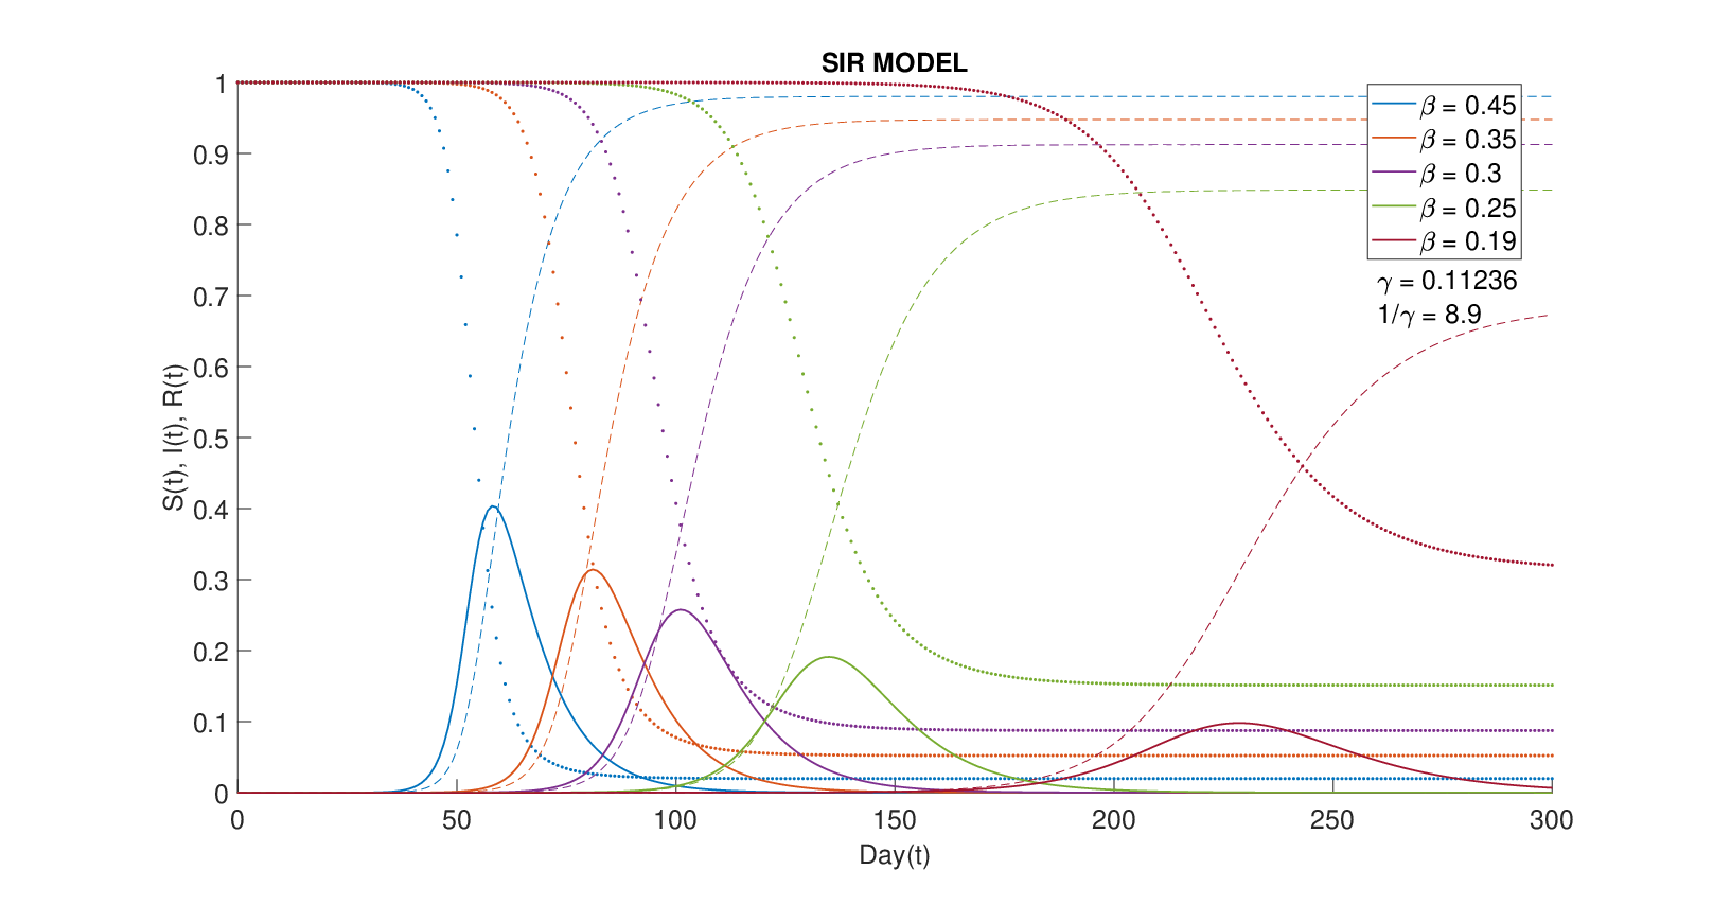
\includegraphics[width=0.48\linewidth]{0_introduction/images_introduction/sir_multipli_beta}} \\
	\caption[SIR dynamic example]{SIR system numerical solutions. Figure a) shows the evolution of compartments in the case of an epidemic. The violet dotted line represents the time-dependent $R_0(t)$. It can be seen that when this parameter is equal to $1$, the number of infected reaches its maximum value. In b) are presented different evolutions of the disease varying only the $\beta$ coefficient. The smaller its value the flattened and the more delayed the infectious curve is.}
	\label{fig:sir_example}
\end{figure}
Other two interesting quantities to consider when a new disease appears are the rate of increase of the infectious and the final size of remaining susceptible at the end of the epidemic. There is a large difference when a population suffers from an epidemic if this ends rapidly because a lot of people get sick or if this number can be controlled, and the infectious curve is flatter. A strategy to flatten the curve can reduce the contact between susceptibles, actuating social distancing or avoiding contact with infected, implementing quarantine measures. These are two simple examples of actions that reduce the value of $\beta$. Another countermeasure is represented by vaccination. Its immediate effect on the epidemic is to remove susceptibles people, so the disease can afflict only a small group and be quickly extinguished. 

\subsubsection{Stochastic models} 	
This is a group of models deriving by the mean-field, but using a different mathematical approach.
In this typology, the transition from one state to another is determined using a function of probability.  Conceptually are derived using the same framework used with ODE models. They are useful when the disease to study has a lower number of infected or if there is a connection between the epidemic outcome and changes in individual dynamics. This is called demographic variability, and it concerns changes in transmission, births, recovery, or deaths within the population. Using stochastic models with Monte Carlo simulations can be useful to investigate epidemic models on networks \cite{Allen2017}. 
The two most important types of models using this approach consider the time variable as continuous, $t \in [0, \infty) $and then the state variable is either discrete (Continuous-Time Markov-Chain) or continuous (Stochastic Differential Equations).
Referring to the SIR model to make a simple example here the S and I compartments are modeled as random variables. The probability of individuals changing groups depends on infection and recovery, the possible events that can occur. It is called transition probability. 
In a Markov chain approach the transition probability is discretized, and there is no dependence on the history of the epidemic to know how it will evolve at time $t + \Delta t$. It is necessary to know only the current state of the process at time $t$. 
In the Stochastic differential equation, the random variables are continuous. 

\subsection{Networked models}
\cite{Newman2002}, \cite{VanMieghem2009}, 


\subsection{Agent-based models}

VEDI E AGGIUNGI ANCHE \cite{Tizzoni2014}

Agent-based models are an alternative technique used to represent disease evolution. This approach is implemented based on the observation of spontaneous connections made by individuals. The evolution of a disease is considered over complex and realistic networks. The focus of this type of model is to understand how the network structure influences the epidemic by observing parameters such as the rate of spread.

In this framework, the nodes of the graph represent individuals (with all the properties that the modeler deems relevant for the study), while the edges represent interactions between people. Nodes can also represent subgroups of people, and using weights on edges makes it possible to characterize the strength of these interactions.

An advantage of this type of model is that it offers a very intuitive approach to epidemic modeling. Using an individual perspective guarantees an immediate interpretation of the model. A precise agent-based model can provide a greater understanding of the illness under consideration and direct information about countermeasures to implement to stop or mitigate its spread. However, to be powerful and capable of performing good analyses and predictions, a lot of information must be integrated into the model. Only if the agent-based model is highly capable of realistically reconstructing a real network can it be a reliable instrument, and achieving this requires very complex work.
\begin{figure}
	\centering
	\includegraphics[width=0.5\linewidth]{0_introduction/images_introduction/agent_based}
	\caption[Agent based network representation]{Agent based network representation}
	\label{fig:agentbased}
\end{figure}

%%

An example of a possible mathematical implementation of this class of models is now briefly presented. One possible technique to describe peer-to-peer contact in a graph structure is realized through a probabilistic framework. Here, assuming a total of $n$ agents in the model, spread processes can be described as a function of probability. Using Markov processes, each agent has a certain probability of transitioning from one state of the disease to another. To calculate the value of these probabilities, both the information derived from the network structure and parameters related to the disease, such as infectivity and recovery rates, are used. In this way, a stochastic evolution model of the processes is developed.

Considering an SIS model described with a Markov process: it has a dimension of $2^n$, while implementing an SIRS model requires a dimension of $3^n$. Because the size of models developed in this manner becomes rapidly enormous, a mean-field approximation is employed. It is based on the assumptions of a network composed of a sufficiently large number of agents and on the independence of these nodes. With this technique, by taking expectations, the transition rates of individuals are approximated. Using these approximations, the boundary values of the agent's probability of infection can be determined at each time step \cite{Hernandez_Vargas_2022}.

\subsection{Multilayer systems and networks} 

AGGIUNGI ANCHE \cite{Wang_2019}

The complex dynamic of interactions existing in the real world, develops in multiple patterns, with complicated relationships. This connection can change over time, and using the theory of multilayer systems it can improve the comprehension of such complexity. Additional information can be added to the model, for example, different types of interactions, like physical contact or information sharing, time dependency coefficients, or reliance between different parameters in nature, creating cause-effect relationships. 
It is a more recent development of the research, the traditional network theory was revisited, to create a framework that can include multiple networks, that evolve and influence each other \cite{DeDomenico2016} and can be helpful to manipulate complex systems like human relationships. Some interesting results obtained are the possibility that the onset of one disease can depend on the onset of the other one. There can be regimes in which the criticality of the two dynamics is interdependent and others in which the critical effect is only one-directional \cite{DeDomenico2016}. 
One possible way to develop models with this structure is to imagine that each layer represents a different type of interaction. An epidemiological example is a layer in which the physical contact between people is simulated and another represents social structure, the network of relations that every person has. This instrument provides a natural representation of coupled structure and dynamical processes. It has been presented in multiple works in the past years, for example in CITA. 
The dynamic realized in multiple systems can be single or coupled. In the first, there is a top layer with its dynamic evolution running on top of a multilayer network. The coupled structure instead is the one in which the phenomena described in each layer evolve with the influence of what is happening in the other. 
Multilayer networks have multiple dimensions of connectivity, called "aspects" and they have to be considered simultaneously. 
They can also be considered with two different mathematical structures. 
\begin{figure}[]
	\centering
	\includegraphics[width=0.6\linewidth]{0_introduction/images_introduction/multi_layer}
	\caption[Multi-layer network]{Representation of a multiplex structure. The figure is taken by the work of \cite{Granell2013} and shows the network implemented in their model. There is an awareness and an epidemic layer. In this case, the node connected with the interlayer connection represents the same individual.}
	\label{fig:multilayer}
\end{figure}

The first uses the same set of compartmental structure and mean-field models presented in the section before \ref{subsec:mean_field}. Here, from a mathematical point of view, there is no such difference in the manipulation and analysis of the system. The distinction relies on the meaning of the compartments and parameters created and on the dependence of the coefficients, which can be time and state-dependent.

The second option considers an agent-based structure. Here, considering a graph structure, composed of nodes and links between them, it is possible to classify three types of edges:
\begin{itemize}
	\item intra-layer edges, the connection of nodes on the same layer.
	\item inter-layer edges, the connection between a replica of the same node, but lying on a different layer of the structure;
	\item inter-layer edges, but coupling nodes representing distinct entities. 
\end{itemize}

A possible representation is done using a $4^{th}$ order tensor or coupling a set of adjacency matrices, called "supra-adjacency matrices". The feature that can be studied is the structural properties of the network, depending on how the various layers are coupled together. The presence of clusters or most central nodes is also important.

 
%%%%%%%%%%%%%%%%%%%%%%%%%%%%%%%%%%%%%%%%%%%%%%%%%%%%%%%%%%%%%%%%%%%%
\chapter{Review of epidemiological behavioural and opinion models in literature}
%NUOVO TESTO
The scientific community's interest in epi-behavior models has existed for several years. Initially, as noted by \cite{Bauch_2012_overview}, the behavioral aspect of epidemiology was not given significant attention. Its development has been a gradual process, resulting from years of evolution in research.

In fact, in the initial works \cite{kermack1927}, the focus of scientists was primarily on describing the evolution of diseases. The resulting models did not account for the effect of behavior; the population was considered homogeneously mixed, leading to random contact between susceptibles and infectives \cite{Hernandez_Vargas_2022, Mata2021}. 
It was only later, as epidemiological models proved effective and reliable in describing and predicting disease spread, that interest among policymakers grew. Tools capable of integrating real data with epidemiological models emerged, aiding decision-making on matters such as the duration of school closures or travel restrictions, as described in \cite{Bauch_2012_overview}.

Furthermore, new categories of models have emerged, such as agent-based models, networked models, and multi-layer/multi-system models. Despite their differing approaches, these models aim to integrate various population characteristics—such as contact structure, age distribution, and movement patterns—to address the limitations of the original homogeneity assumption \cite{brauer2012mathematical}.
This focus on societal composition and behavior naturally stems from the desire to use modeling tools as a reference for decision-making in safety and health. 
One possible approach to incorporating changes in the structure of models that describe aspects of behavior or population composition is to do so implicitly.

In these models, the behavior of the population is implicitly considered by integrating time-variable parameters that capture changes in societal behavior. This approach represents the classical modeling technique used in the formulation of epidemiological models. Examples of studies that have utilized this methodology for analyzing COVID-19 include \cite{Giordano_2020, Dehning_2020, Proverbio_2021}.

Although models developed in this way have proven to be powerful tools for generating insights about disease dynamics and providing recommendations to policymakers, they fall short in their ability to accurately reconstruct how populations behave during an epidemic outbreak. The desire to explore this aspect and develop a framework capable of simultaneously simulating both behavior and disease diffusion—where each mutually influences the other—has driven the development of a specific research field dedicated to behavioral epidemics.

But how can behavior be integrated into pre-existing epidemiological theory? To better address this question, we follow the classification proposed in \cite{Funk_2010}, which offers a possible subdivision of behavioral literature based on the different approaches that most articles focus on. Three major categories emerge:
\begin{itemize}
	\item The source of information used to make decisions;
	\item The type of information used to make decisions;
	\item The effect of behavioral change on the dynamic described by  the model. 
\end{itemize}
When analyzing the source of information, there is a clear distinction between works that assume governments and populations base their decisions on precise data, such as the number of infected individuals (prevalence), and those that consider more informal sources, such as conversations between people, public opinion, or media representations of the situation \cite{Bulai2023}. These media sources include both traditional outlets like television and newspapers, as well as newer platforms like social networks.
This distinction highlights the diversity in how behavioral factors are integrated into models, reflecting the varying degrees of reliability and influence these sources have on decision-making processes during an epidemic.


Regarding information quality and the negative effect of misinformation spreading within the population, an example is the fear of vaccination \cite{Kahan_2013}. Several works analyze the effect that fear of vaccination has had on the spread of infection \cite{Bauch_2012_game, Epstein_2021}.
An example of how this phenomenon can arise is the story of an article originally published by a prestigious source. Even though the thesis presented in this work was later proven wrong by the scientific community \cite{wakefield1998retracted}, the negative impact in terms of spreading fear about vaccines has persisted and, in many cases, has become deeply ingrained. In this specific case, it caused a decrease in herd immunity and a resurgence of measles \cite{Bauch_2012_overview}.


After introducing the impact that information quality may have, another interesting aspect is related to the different types of information used in model development. Some articles focus on the effect of media on behavior \cite{Collinson2014, Misra_2011}, while others consider peer-to-peer conversations, information exchange, and beliefs among individuals \cite{Tyson_2020}. These are completely different approaches, even though they aim to achieve the same effect: simulating the evolution of people's opinions and behavior. Using media involves hypothesizing that the population is influenced by a few "central" information nodes, so the same news, data, or future predictions are shared with everyone. In contrast, models that use personal information exchanges can depict a scenario where many different ideas about the disease situation circulate simultaneously.
Another concept used in models that simulate a sort of "collective consciousness" is referred to as "awareness" \cite{Funk2009}. To model how awareness spreads in the population, it is often treated like a disease \cite{Silva2019, Granell_2013, Granell2014, Kabir_2019, Zuo_2021, Wang_2019}. Although there are differences, the main idea is that theories and concepts about a certain topic can spread among people, which can be considered at a higher level as a unified opinion. For example, there may be many different personal positions on how to respond to a health emergency like COVID-19, but it is possible to abstract the various opinions and reconstruct what the majority of people, or macro-groups, ultimately feel. They may either be more cooperative and in favor of following guidelines issued by authorities or more focused on their well-being and inclined to act independently.
This process can be related to opinion formation studies, which aim to understand how people form their ideas \cite{Devia_2023, Devia2022} and also analyze the possible formation of opinion distributions, such as perfect consensus, consensus, polarization, clustering, or dissensus.
 
\chapter{Old review}

The development of a epidemiological model, that can capture the evolution of a disease influenced by the behaviour of individuals, begins from a study and review of the most significant works already present in this research topic.
These are the different main type of model that have been investigated:
\begin{itemize}
	\item deterministic/mean field models
	\item opinion models
	\item multilayer networks
	\item opinion-disease models	
\end{itemize}

Now it is presented for each of them, the main aspect and knowledge, useful for the development of my model.   

\section{Opinion models}
In the analysis performed by Wang \cite{Wang_2019}, are presented mechanism implemented to explain co-evolution spreading in complex network. The principal methodologies created over time are threshold model, that can use a linear threshold or a “Watts threshold”. Here each node has a random different threshold, based on a certain distribution. Using a threshold means that a node change opinion on the basis of its neighbours’ belief. The shape of the network is then fundamental for an opinion to spread. The best scenario is the one in which there is a low degree of randomness, and the network is regular. Also, cluster can have a reinforcement effect, if they are sufficiently connected to the resto of the graph. Their work then report analysis based on competition or cooperation of opinions “contagions”. And a SAR model is presented. Similar to a SIR, here the meaning of letter A is “adopted”. It means becoming convinced of a certain opinion, but with a probability or rate to then return to the previous behaviour. 

Also the work of \cite{Nunner2021} define and test some different models based on trade-off between the benefit of having connections and the penalty for acquiring infections. It is showed that when the behaviour of people depends on maximizing their net benefit, the individual risk perception plays an important role in the formulation of a cost function. The models derived with this so called co-evolutionary approach, have an overall dynamic very correlated between the two strati: it is a feedback loop between infection spreading, people behaviour adaptation and consequently structural modification in the network.


\section{Multilayer network}
One work based on feedback between two networks concatenated is the one performed by Peng et all, \cite{Peng2021}. Here there is explained a model based on two graphs, where one simulates the evolution of a disease, using a SIR or SIRS dynamic, and another explicit the behaviour of individual in a UPAU network. U means uninformed, P pro-physical distancing and A anti-physical distancing.  In this network the people’s conduct influence the $\beta$ coefficient of the epidemic diffusion. They demonstrate the effectiveness of having an opinion in reducing the negative effect of a disease and that lengthening the duration time for which an individual maintains opinion can help suppressing the transmission.
Study the effect of competition in a multilayer network is the objective of Teslya et all research \cite{teslya2022}. At cause of interpersonal communication individual can change their opinion. They are divided in two main groups, positive or negative w.r.t health conduct. Here is also inserted an influence due to assortatively when contacting with others. Their principal results further than the fact that opinion influence disease, is realizing a model in which the two opinions can coexist at equilibrium. There can be oscillation of prevalence due to increased transmissibility of infection. In SIR model they demonstrate a reverse correlation between the rate of social contact and the peak magnitude of infectious. The causes of oscillations in the disease dynamic are a high infection rate and a pronounced difference in infection rate between individuals with different opinions. The others important factors are the high-rate opinion exchange and high sensitivity of population to prevalence. 
In the article \cite{ Alvarez_Zuzek_2017} the opinion about vaccination is taking in consideration, into a SIR+V mean field model. Conversating is the mean used by individual to modify their opinion. With a very positive opinion susceptible individuals can choose to take the vaccine. Interesting they use a r factor to describe the extremism in opinion. Varying this coefficient, they observe that the best scenario for delay the development of an epidemic is the one where the society is neutral. So, when there aren’t compromise or persuasion, but the conversation is based on “rational” arguments.  Another works analysing two competing opinion is \cite{Epstein_2021}. Here population is sensitive to both fear of vaccine and disease. These two interact and the vaccination grow rate increases only if the fear of the disease is larger than the of vaccine.  The infection curve is very influenced by the presented dynamic, and the best scenario is obviously the one in which the fear of vaccine does not exist. However, in the case where the two fears coexist there is an improvement in the number of infected, for multiple infection waves.
The work by Auld \cite{Auld_2003}, reflect an observed characteristic in society: pessimistic expectations over the future induce a more risky behaviours. This conclusion derives observing and simulation evolution correlated to the news about a vaccine. This knowledge causes a decrease in infection rate before the vaccine becomes available. Then there is a return to normal behaviour. If there are not information, pessimism cause more risky behaviour. 
In \cite{Sontag_2022} there is another SIR and opinion model, with population that is divided in trusting and distrusting. They add in the model the effect of fading and a global force, that simulates central interventions. The main interesting conclusion of their work is that strong public intervention have a similar effect to the network to the ones obtained if the population is composed of trusting and compliant individuals. However, higher percentages of distrusting cause the model to pass a phase transition where outbreaks cannot be suppressed. 
A different approach in using a multilayer network is the one realised in \cite{Turker_2023}, where the social structure of a town is re-created. Every layer describes the places populated by individuals: from house, to work, distinguishing between different type of work, and considering a level for friendship. Each person is present to more than a layer and, in each layer, relates to different agents, based on the social group’s provenience.  Using this approach, they have found that the level in which is easier for an outbreak to develop is the one associated with friendship. Here the interaction is closer with others, the security level is lower. For this reason, a lower value of transmissibility rate $\beta$ is sufficient to have an epidemic with many susceptible involved. 

\section{Opinion-disease model}
The work done by Funk and its colleagues \cite{ Funk_2010}, it is very interesting: they collect and explain systematically the behavioural reaction of population in response to a pandemic. They classify the human behaviour subject to different possible sources of information. An information can be global available or local. This reflects the way it radiates or if develops in social cluster. Another important difference is related to objectivity. Certain information is based on belief and can change with time. This typology can be influenced by the social connections of an individual or by the influence of external agents, like media. Cognitive bias also can have an impact on our opinions: amplification, confirmation, anchoring bias. They then focus on the influence of self-initiated action in the control of disease diffusion. When an individual change its behaviour, form a modelling point of view this can influence: its probability to change state (from S to I for example). The value of $\beta$ or $\gamma$. Modification in the contact network, with a self-isolation or adherence to more cautious conduct. Fear has an important role in how people face epidemic. Due to this emotion, people can decide to get vaccinated for example (or not, if they are more frightened by vaccines). Another phenomenon observed and influenced by fear is saturation. When there is many infectious people tend to decrease their number of contact and this cause a decrement in the I curve.  Another multilayer network with two opinion, 0 where individual not take precautions and 1 where the protective measures are used, is presented in \cite{Frieswijk_2022}. This model is associated to a SIS disease one. The article studies the stability of asymptotically equilibria of the system. Assuming different value of a parameter used to describe risk perception they found a set of final possible states. The most interesting is a stable asymptotical equilibrium in which there is a periodic epidemic outbreak and a consequently population behaviour response, changing behaviour to a safer.
An analysis of people choices about vaccinations is done by \cite{Bauch_2012}, they study the feedback between the positive effect due to vaccination and the fear of being vaccinated. In fact, thanks to vaccines, the disease incidence can become very low, and the perception of risk related to them can seem larger. They implemented an approach based on game theory and using social learning.
A possibility to integrate the effect of opinion in the dynamic of an epidemic, is creating different subgroups of susceptible. They are separated according to their level of opinion, and the less they belief in use of NPI, for example, the higher probability of being infectious they have. This is the approach used in \cite{Tyson_2020}. They also implemented different functions describing the influence between opinion and the possibility to become infected. 
The influence of media has also been analysed. This is interesting, because it’s a communication channel that can be used by government, and so it is an available control measure that can be implemented, to try control the behaviour of population.  For example in \cite{Collinson2014} a parameter depending on I value simulates the effect of media covering the news about the disease. Increasing the number of infectious cause, the creation of news and other media about it. These can have as effect to induce more people practice social distance for example. Study both the effect of media, see as a central node of communication joined with opinion evolution is done in \cite{Granell_2014}. Nodes co-exist into two layer, one for disease spreading and one for awareness, (unaware-aware-unaware model). In their application the awareness process without media, must reach a certain level on the transmissibility of awareness to influence the onset of epidemic. Instead, with an influence of media, greater than zero, this “metacritical” point disappears. A central broadcast, even with a small communication influence power, as a direct effect on all the network dynamic. 
\part{Behavioral-Disease Model}
\label{part:the_model}
\chapter{Model development and justification}
\label{ch:why_new}
Because the main contribution of this thesis is the development of a new multi-system model, understanding the reasons that led to its development is crucial.
Otherwise, the reader might question: "Why not use an already developed and analyzed model?"

The primary answer lies in the observation made while studying the literature: the connection between empirical data and epidemiological models is often missing. Most works relating social and epidemiological aspects are purely theoretical models based on ad-hoc assumptions; probably, because constructing a framework grounded in empirical data related to individual behavior is challenging \cite{Nunner2021}, and, until the COVID-19 pandemic, data on this topic were scarce.

The availability of research such as the one conducted by Meta during the COVID-19 pandemic \cite{Astley_2021} serves as a major source of inspiration and data. This research allows exploration of different behaviors related to how people react to and manage the necessity of living with an infectious disease. It also provides this valuable information as a dynamic time series.

Often, what emerges from this data is the non-linear dynamic evolution of behavior. While many models do not incorporate this characteristic \cite{huys2010nonlinear}, this feature is here addressed.
\begin{figure}[ht]
	\centering
	\includegraphics[width=0.8\linewidth]{1_corpo/figure/Fig2cut}
	\caption[Mask wearing evolution]{The evolution of mask wearing behaviors during the COVID-19 pandemic. Figure from \cite{Proverbio_Tex_2024}.}
	\label{fig:mask_wearing}
\end{figure}
The behavioral-epidemic mean-field model we developed aims to interconnect these two features, linking the theoretical framework with empirical evidence. Often, in other works, this connection is realized using proxy models that attempt to reconstruct agent behavior, spatial motion, or opinion datasets extrapolated, for instance, from social networks, as done in \cite{Anderson_2019,Zino_2021}. The problem with these approaches is that people's opinions do not always align with their actual behaviors, and the lack of a necessary and direct correlation between the two is another concept the model attempts to overcome.

For example, consider the evolution of mask-wearing behavior in different European countries during the COVID-19 pandemic, as shown in Figure \ref{fig:mask_wearing}. It is immediately evident that, at a certain point, there is a sharp increase in the use of this self-protective device, resembling a step function. This effect results from regulatory prescriptions introduced by authorities, and behaviors closely follow the evolution of these stringency measures.

Such phenomena have been incorporated into the model development using a coefficient parameter, $\psi$, to represent the effect of centralized interventions and modify the basic persuasion rate of different behaviors. Additional empirical evidence supporting the development of the model can be found in \cite{Proverbio_Tex_2024}. 

\begin{figure}[ht]
	\centering
	\includegraphics[width=0.6\linewidth]{1_corpo/figure/Model_behav_epidemic}
	\caption[Epi-behavior model]{Representation of the model with individuals divided into different behavioral categories, each of which can correspond to a specific disease state, except for the Heedless group, which is characterized solely by Susceptible individuals.}
	\label{fig:modelbehavepidemic}
\end{figure}

To introduce the model and begin its description, the next chapter first presents and analyzes the two layers that together form the complete model: a SIRS epidemic model and a behavioral model consisting of three compartments: Compliant, Against, and Heedless. Then, the full model is presented, described and analysed in Chapter \ref{ch:epi_behav_model}.
Then the full model is presented, described and analysed. 
The full model comprises seven compartments, as the heedless behavior is not possible for individuals that are infected or recovered. This assumption stems from the reasoning that it is highly improbable for an individual to act heedlessly when infected (unless, potentially, when completely asymptomatic). Figure \ref{fig:modelbehavepidemic} provides a compact representation of the population subdivision.

Infection can be transmitted across all three behavioral groups, but the Compliant group is more cautious. A parameter, $\rho$, models their reduced probability of being infected, while another parameter, $\epsilon$, accounts for their compliance with self-isolation while infectious. This reduces the number of infected Compliant individuals ($I_C$ in the model equations that will be presented in the next chapter \ref{ch:epi_behav_model}) contributing to new infections in the epidemic layer.

Behavior is "transmitted" through peer-to-peer influence with strenght parameters ($k_i, i = \,1,...,6$), with $i$ the number of compartments either Compliant or Against, and fatigue parameters ($\lambda_i$) are included to model the dropout rate caused by the difficulty of maintaining a certain behavior over time.

For the epidemic components of the model, classical coefficients are used: $\beta$ (transmission rate), $\gamma$ (recovery rate), and $\delta$ (immunity waning rate).
 

\chapter{Epidemic model and Behavioral model alone}
\label{ch:model_alone}

To develop a multi-system model that combines an epidemiological layer with a behavioral one, we first present the dynamics of each layer independently. We briefly introduce the SIRS model, focusing primarily on the reasons for its selection. Then, the Heedless, Compliant, Against behavioral model is introduced, simulated, and analyzed. Understanding the underlying dynamics of this model is crucial for gaining insight into the complex interactions that emerge within the multi-system model.


\section{SIRS model}
\label{sec:SIRS}
To describe the epidemic evolution, a  SIRS model is implemented. It is an extension of the most famous SIR discussed in Section \ref{subsec:SIR}. Its main addition is the possibility for individuals to become again susceptible after a certain period of time beyond the end of the infection due to waning immunity. There are four main characteristic parameters in this model:
\begin{itemize}
	\item $\beta$ is the transmission rate parameter for person-to-person
	contact.
	\item $\gamma$ is the recovery rate.
	\item  $\delta$ is the rate at which immunity wanes following recovery.
	\item  $\mathcal{R}_0$ is the reproduction number, similar conceptually to the one presented in SIR model, but function of $\beta, \gamma$, and also $\delta$. 
\end{itemize}
A SIR-like model is chosen because of its ability to describe diseases like COVID-19; the literature provides numerous examples that use this model \cite{Dehning_2020, Li2022}. The SEIR model could also be a viable choice due to the relevance of the "Exposed" compartment, which effectively captures the disease progression for infections such as COVID-19. In these cases, an incubation period occurs after exposure before symptoms appear and the individual becomes contagious. However, this compartment was excluded because it has been shown \cite{Dehning_2020} that a simpler SIR model can still accurately represent the disease dynamics. When comparing model simulations with real data, a delay can be incorporated to account for the lag between symptom onset, testing, and reporting. This delay reflects the time needed for symptoms to manifest, conduct testing, and report cases to relevant authorities.
The differential system of equations describing the model are
\begin{equation}
	\label{eq:SIRS_eq}
	\begin{cases}
		\frac{ds}{dt} = -\beta s i + \delta r \\
		\frac{di}{dt} = \beta s i -  \gamma i \\
		\frac{dr}{dt}= \gamma i -  \delta r\\
	\end{cases}
\end{equation}
with $s(0) = s_0 \ge 0$, $i(0) \ge 0$ and $r(0) = 0$. The mass conservation assumption holds so $s(t)+i(t)+r(t) =1$.
The model includes the possibility of reinfection, which is important when studying long-term scenarios. Considering the effect of individual behavior on disease progression, two critical phases are hypothesized to influence this evolution: the initial stages of the epidemic and the period following the first peak.

In the initial stages, the SIRS model behaves similarly to a typical SIR model, because reinfection is unlikely to occur in a short time frame. However, over time, as reinfections become possible, individual attitudes and behaviors increasingly impact the disease spread.

\begin{figure}[ht]
	\centering
	\includegraphics[width=0.6\linewidth]{1_corpo/figure/r0/sirs_figure}
	\caption[SIRS simulation]{Simulation of the SIRS model. The parameters of the model, which meaning is presented in section \ref{sec:sir_presentation}, are chosen to resemble those of the initial stages of the COVID-19 pandemic \cite{data_R0_covid} and are the same as those used for simulations with the full epi-behavioral model.}
	\label{fig:sirsfigure}
\end{figure}

\section{Behavioural model}
\label{sec:behavioral_model}

The development of the behavioral model builds on several works already presented in the literature. In particular, the following mechanisms are considered to be the most relevant:
\begin{itemize}
	\item The competition between two opposing behaviors/opinions, driven by peer pressure \cite{Epstein_2021}. The implementation is inspired by the Unaware-Aware-Unaware opinion model class \cite{Zuo2022, Peng2021}, refer to Section \ref{subsec:individual_state} and \ref{subsec:multisystem_models}, for how the compartments are linked together and for the idea of social pressure between individuals.
	
	\item Non-compliance viewed as a form of social contagion \cite{Bongarti2023}.
	 
	\item The fatigue mechanism, due to which maintaining a certain behavior for long leads to a spontaneous loss of compliance \cite{Epstein_2021}.
\end{itemize}

To integrate all these aspects into a mean-field model, the first step is to define the compartments used to segment the population. The population is divided into three compartments: Heedless, Compliant, and Against, denoted respectively as H, C, and A. The meaning of each compartment is as follows:
\begin{itemize}
	\item[\textbf{$H$:}] Individuals who behave without much regard for guidelines and are careless about the risks associated with the infection.
	\item[\textbf{$C$:}] Individuals who actively seek to avoid becoming infected or spreading the virus by following guidelines and taking precautions.
	\item[\textbf{$A$:}]Individuals who do not consider the infection a risk to their safety and do not use protection or modify their behavior during the epidemic. They disregard risk-mitigating guidelines and do not align with safer behaviors as the epidemic unfolds.
\end{itemize}

\subsubsection{Initial conditions}
As an initial condition, the hypothesis is that most of the population is in the Heedless compartment. This assumption is based on the idea that when a new disease emerges, it is poorly understood, and the population has limited information about it. The hypothesis is that people in the Heedless compartment may be clueless about the risks of becoming infected. This lack of knowledge causes them to maintain their usual behavior, making them susceptible to infection. This assumption is also supported by data and literature \cite{Usher_2020}. As an example of this initial configuration, the case of COVID-19 in Italy is considered. In the early stages of its spread, when the disease was primarily affecting China, it was not viewed as a significant threat by most of the population in Western countries. It was perceived as a distant issue affecting a faraway nation. Therefore, when the epidemic reached Europe and Italy, both the population and the government were caught off guard. There was an initial delay in the implementation of countermeasures, as well as in the dissemination of reliable information about the disease progression to the general public.

In addition, there are two opposing behavioral groups, which in the initial phase of the dynamic comprise a small fraction of the population: Compliant and Against.

The Compliant group actively seeks to reduce their chances of becoming infected or infecting others. They adopt self-protection measures such as wearing face masks, sanitizing their hands, and voluntarily limiting their presence in public spaces to reduce contact with others.

In contrast, the Against group consists of individuals who, for personal reasons—such as anti-scientific beliefs, low trust in policymakers, or other concerns—do not take action to minimize their chances of infection or the possibility of infecting others. This category encompasses phenomena such as: 
\begin{itemize} 
	\item vaccine denial; 
	\item misinformation spread; 
	\item denial of the existence of the disease; 
	\item distrust of doctors and government policies. 
\end{itemize}

The inclusion of the Against compartment stems from the fact that, especially in the early stages of a new disease outbreak, there is often a lack of reliable knowledge. As documented by \cite{McCormack_2020}, this can lead to the spread of false beliefs in the population. It has also been demonstrated \cite{owid-vaccine-skepticism} that misinformation, especially when associated with fear, can have lasting effects. A notable example is the belief that the measles, mumps, and rubella (MMR) vaccine can cause developmental disorders in children. Despite the fact that the original publication making this claim has been scientifically discredited \cite{wakefield1998retracted}, this idea remains popular and has contributed to a rise in vaccine skepticism \cite{owid-vaccine-skepticism}.

\subsubsection{Social contagion dynamic}
The evolution of the model is governed by two principal mechanisms: \begin{itemize} 
	\item Heedless individuals transition to either Compliant or Against compartments. 
	\item Compliant and Against individuals return to the Heedless compartment. 
\end{itemize}
\begin{figure}[ht]
	\centering
	\includegraphics[width=0.72\linewidth]{1_corpo/figure/behavior_model_figure}
	\caption[Behavior model]{The figure visualizes the developed behavioral model, featuring three compartments: Heedless, Compliant, and Against, abbreviated as H, C, and A. The arrows indicate the inflows and outflows between these compartments.}
	\label{fig:behaviormodelfigure}
\end{figure}
The first mechanism is driven by peer pressure: the size of each group and its level of persuasiveness are the parameters that govern this process. It is mathematically modeled similarly to person-to-person disease transmission, as seen in the SIR-like mean-field model described in Section \ref{subsubsec:p2p_transmission}. Instead, the return to the Heedless compartment is modeled as a spontaneous decay process: individuals naturally leave the Compliant and Against compartments and return to Heedless, transitioning spontaneously depending on the level of fatigue associated with maintaining the behavior.The flow between an intermediate compartment, represented by $H$, rather than a direct transition between $A$ and $C$ (and vice versa), is a modeling choice stemming from the idea that heedlessly can, when a new disease appears, signify lack of awareness about it. Over time, it can represent instead the state of people after a period of coexistence with the disease, where the fatigue of maintaining compliance increases, or when indifference toward the disease grows.
To describe these transitions, different coefficients are introduced. The $k_1$ and $k_2$ are persuasion rates, while $\lambda_1$ and $\lambda_2$ represent fatigue rates. Their meanings are as follows: \begin{itemize} 
	\item $k_1$: persuasion rate from Heedless to Compliant; 
	\item $k_2$: persuasion rate from Heedless to Against; 
	\item $\lambda_1$: rate at which the Compliant behavior is abandoned due to fatigue; 
	\item $\lambda_2$: rate at which the Against behavior is abandoned due to fatigue. 
\end{itemize}

The resulting differential equations describing the model dynamic are:
\begin{equation}
	\label{eq:behavioural_eq}
	\begin{cases}
		\dot{H} = -k_1 H C - k_2 H A + \lambda_1 C + \lambda_2 A \\
		\dot{C} = k_1 H C -  \lambda_1 C \\
		\dot{A} = k_2 H A -  \lambda_2 A\\
	\end{cases}
\end{equation}
We assume population mass conservation, meaning that the relationship $H + C + A = 1$ holds. Additionally, the initial conditions described in the previous section are translated as follows:
\begin{equation}
	\begin{cases}
		H(0) = 1 - C_0 - A_0\\
		C(0) = C_0 > 0\\
		A(0) = A_0 > 0\\
	\end{cases}
\end{equation}

\subsubsection{Behavior conversion number}

To simplify the understanding of the system underlying dynamics, an analogy can be drawn with the reproduction number in epidemic models. By examining the system equations \eqref{eq:behavioural_eq}, a relationship can be identified. From both the second and third equations, we can isolate the two coefficients (specifically $k_1 , \lambda_1 $, and  $k_2 , \lambda_2 $)  and derive a new parameter, called "Behavior Conversion Rate", $\mathcal{B}$. This rate is the result of the ratio between the persuasion rate and the fatigue decay rate, and can be viewed as a measure of the transmission potential of social contagion. The general formula to calculate it is:
\begin{equation}
	\mathcal{B}_i =\frac{ k_i }{\lambda_i}  \qquad \text{with } i = 1, \text{or } 2.
	\label{eq:behave_rate}
\end{equation}
In the model presented here, $\mathcal{B}_1$ represents the Behavior Conversion Rate associated with the Compliant compartment, while $\mathcal{B}_2$, is associated with the Against compartment. The results of different numerical simulations are now displayed to demonstrate how the relationship between these two values influences the evolution of social contagion.

\subsection{Model simulation}
To represent different dynamics, four main cases are now presented. The coefficient values have been set appropriately to highlight different interesting situations in which the system can evolve.

\begin{itemize}
	\item[I] case: $\mathcal{B}_1, \mathcal{B}_2 <1$, $\mathcal{B}_1 >  \mathcal{B}_2$, and $\lambda_1 > \lambda_2$.
	\item[II] case: $\mathcal{B}_1, \mathcal{B}_2 >1$, $\mathcal{B}_1 =  \mathcal{B}_2$, and $\lambda_1 < \lambda_2$.
	\item[III] case: $\mathcal{B}_1, \mathcal{B}_2 >1$, $\mathcal{B}_1 >  \mathcal{B}_2$, and $\lambda_1 = \lambda_2$.
	\item[IV] case: $\mathcal{B}_1, \mathcal{B}_2 >1$ and $\mathcal{B}_1 >  \mathcal{B}_2$, and $\lambda_1 < \lambda_2$.
\end{itemize}

The values $k_1$ and $k_2$ can be calculated from the formula of $\mathcal{B}_1$ and $\mathcal{B}_2$.

Figure \ref{fig:model__behavior_sim_1}a shows that, when both Behavior conversion numbers are less than one, social contagion does not spread: even though, in this case, the Compliant and Against compartments together represent $60\%$ of the total population at the beginning of the simulation, they clearly tend to zero over time. In contrast, Figure \ref{fig:model__behavior_sim_1}b shows the case where the two $\mathcal{B}$ values are equal and greater than one. To emphasize the importance of the relations between fatigue and persuasion rate, it is shown that, even if the conversion numbers are equal, (i.e. $k_2$  is lower than $k_1$=), the Compliant compartment becomes the majority group by the end of the simulation. Here the Against do not tend to zero, but there is a rather stable flow between the Compliant and Against compartments, through the Heedles state, such that
none of the compartments becomes empty.

\begin{figure}[ht]
	\centering
	\subfloat[][\emph{$\mathcal{B}_1, \mathcal{B}_2 <1$, $\mathcal{B}_1 >  \mathcal{B}_2$, and $\lambda_1 > \lambda_2$.}]
	{\includegraphics[width=0.48\linewidth]{1_corpo/figure/behavioural_equilibrium/behavior_B1_B2_less_1}} \quad
	\subfloat[][\emph{$\mathcal{B}_1, \mathcal{B}_2 >1$, $\mathcal{B}_1 =  \mathcal{B}_2$, and $\lambda_1 < \lambda_2$.}]
	{\includegraphics[width=0.48\linewidth]{1_corpo/figure/behavioural_equilibrium/behavior_B1_equal_B2}} \\
	\caption[Behavioural model simulation first]{Behavioral system dynamics first two cases (I and II). In the left panel there is the case in which both $\mathcal{B}_1$,$\mathcal{B}_2$ are less than one. The system tends to an equilibrium in which all individuals tends to the $H$ state. In the right panel, instead the case in which the conversion number are equal, but because $k_1 > k_2$ the Compliant variable becomes greater than the Against one.}
	\label{fig:model__behavior_sim_1}
\end{figure}
\label{subsec:model_behav}

Figure \ref{fig:model__behavior_sim_2} illustrates two other interesting scenarios. On the left, we observe the dynamics when one of the $\mathcal{B}$ values is greater than the other, and both $\lambda$ values are the same: the variable with the largest $\mathcal{B}$ becomes dominant. It is straightforward to understand that this dynamic would also occur if, with the same values of $\mathcal{B}$, the $\lambda$ of the dominant behavior were greater than the other, as a larger $\lambda$ would be compensated by  a higher $k$ (persuasion rate). The right panel, however, presents a particularly intriguing situation. Here, $\lambda_1$ < $\lambda_2$, combined with $k_2 > k_1$, leads to an initial rapid spread of the Against group, even though $\mathcal{B}_2 < \mathcal{B}_1$! It is only after some time that the system evolves to the final equilibrium, which is the same as in the left scenario, as the $\mathcal{B}$ values are the same in both simulations.

\begin{figure}[h]
	\centering
	\subfloat[][\emph{$\mathcal{B}_1, \mathcal{B}_2 >1$, $\mathcal{B}_1 >  \mathcal{B}_2$, and $\lambda_1 = \lambda_2$.}]
	{\includegraphics[width=0.48\linewidth]{1_corpo/figure/behavioural_equilibrium/behavior_B1_mag_B2_k1_mag_k2}} \quad
	\subfloat[][\emph{$\mathcal{B}_1, \mathcal{B}_2 >1$ and $\mathcal{B}_1 >  \mathcal{B}_2$, and $\lambda_1 < \lambda_2$.}]
	{\includegraphics[width=0.48\linewidth]{1_corpo/figure/behavioural_equilibrium/behavior_B1_mag_B2_k2_mag_k1}} \\
		\caption[Behavioral model simulation second]{Behavioral system dynamics: the second two cases (III and IV). In the left panel, the scenario depicts Compliant becoming the dominant group, while Against gradually tends toward zero. In the right panel, with the same value for the conversion number but a higher persuasion rate for Against compared to Compliant, the system converges to the same equilibrium as in the left figure. However, it first goes through a phase where the Against group becomes dominant.}
	\label{fig:model__behavior_sim_2}
\end{figure}

\subsection{Equilibrium and stability analysis}
To enhance our understanding of the system, equilibria are computed and their stability is studied. As observed, the system equilibrium values vary according to parameter values. Specifically, the coefficients were combined to produce two Behavior conversion numbers, $\mathcal{B}_1$ and $\mathcal{B}_2$. One way to identify and visualize the system equilibria for a specific parameter set is through nullclines, used in an autonomous system of differential equations (DE)  to sketch the phase plane of the system. In a system of two DE: 
  
\begin{align}
	\frac{dx}{dt} &= f(x,y) \\
	\frac{dy}{dt} &= g(x,y)
\end{align}

there are two types of nullclines: $x$-nullcline, and $y$-nullcline. The $x$-nullcline is the set of points in the phase plane so that $\frac{dx}{dt} =0$, and graphically can be represented as a set of vectors that go either straight up or down. Instead, the $y$-nullcline is the set of points for which $\frac{dy}{dt} =0$. In these points the vectors are horizontal, going either to the left or to the right.

The original system of three equations, \eqref{eq:behavioural_eq}, has been reduced, to better visualize nullclines in a two-dimensional graph, by using the population conservation assumption: $1 = H + C + A$. By substituting the $A$ term as $A = 1 - H- C$, it is obtained a system of two equations with two unknowns:
\[
\begin{cases}
	\dot{H} = -k_1 H C - k_2 (1-H-C) H + \lambda_1 C + \lambda_2 (1-H-C)\\
	\dot{C} = k_1 H C - \lambda_1 C
\end{cases}
\]
To simplify the readability and use a notation more familiar for plotting,  $H, C$ have been substituted with respectively $x, y$. So, the equations become:
\begin{equation}
\label{eq:system_nullclines}
\begin{cases}
	\dot{x} = -k_1 y x - k_2 (1-y-x) x + \lambda_1 y + \lambda_2 (1-y-x)\\
	\dot{y} = k_1 y x - \lambda_1 y
\end{cases}
\end{equation}
The nullclines can be calculated by imposing $\dot{x} = 0$ and $\dot{y} = 0$. For the first nullcline, with $\dot{x} = 0$,

\begin{equation}\\
\label{eq:x_nullcline}
 y = \frac{x(k_2 - k_2 x + \lambda_2) - \lambda_2}{x(k_2 - k_1)+ \lambda_1- \lambda_2}
\end{equation}
and for the second, with $\dot{y} = 0$,
\[x = \frac{\lambda_1}{k_1} = 1/\mathcal{B}_1 \quad \text{or } y = 0.
\]
%The selection of the correct $\mathcal{B}_i$ to use for the second nullcline depends on the comparison between the two reproductive ratio values. Seeing the result of the simulation, it is understood that the larger value should be chosen, as it represents the behavior that will dominate at equilibrium, while the other behavior will tend toward zero. Only in the case where the $\mathcal{B}_1, \mathcal{B}_2 < 1$ this rule does not hold, because the result of the second nullcline found with the formula is out of the domain of existence (i.e $x > 1$, while the Compliant, $x$ is a value comprised between $[0,1]$.)
The existence condition for the first nullcline can be calculated, imposing that the denominator must not be equal to zero:
\[ x \neq \frac{\lambda_2-\lambda_1}{k_2 - k_1} \]
This value can be in the interval $[0,1]$ only if $\lambda_2>\lambda_1$ and $k_2 > k_1$, or $\lambda_2<\lambda_1$ and $k_2 < k_1$. The second nullcline instead, always exists if $k_1 \neq 0$.

\subsubsection{Equilibria of the system}
The equilibrium value can be computed as the intersection point of the two nullclines, from equation \eqref{eq:x_nullcline}. In fact if $x =\frac{\lambda_1}{k_1}$, then $y = 1 -\frac{\lambda_1}{k_1}$.
Instead if $y = 0$, two values are found: $x = 1$, and $x = \frac{\lambda_2}{k_2}$.
The three equilibria, indicated as $Eq_1, Eq_2 $, and $Eq_3$, are then:
\begin{itemize}
	\item $Eq_1 = (\frac{\lambda_1}{k_1}, 1-\frac{\lambda_1}{k_1})$
	\item $Eq_2 = (1, 0)$
	\item $Eq_3 = (\frac{\lambda_2}{k_2}, 0)$
\end{itemize}

\subsubsection{Equilibria stability analysis}
To assess the local stability of the equilibrium points, the Routh-Hurwitz criterion is applied, requiring the Jacobian matrix of the system evaluated at each equilibrium. The equilibrium is locally stable if:
\begin{itemize}
	\item the trace of the Jacobian is negative: tr($J$)$< 0$
	\item the determinant of the Jacobian is positive: det($J$) $> 0$
\end{itemize}
The Jacobian of the system \eqref{eq:system_nullclines} is
\begin{equation}
	J = \begin{bmatrix}
		-k_1 y -k_2 +k_2 y+2 k_2 x- \lambda_2 & -k_1 x + k_2 x + \lambda_1-\lambda_2 \\
		k_1 y & k_1 x - \lambda_1
	\end{bmatrix}
\end{equation}
The trace of $J$ is
\begin{equation}
	\text{tr}(J) = -k_1 y -k_2 +k_2y + 2 k_2 x - \lambda_2 -\lambda_1 +k_1 x
\end{equation}
Its determinant is instead
\begin{equation}
	\text{det}(J) = k_2 \lambda_1 + \lambda_1 \lambda_2 + 2 k_1 k_2 x^2 - k_1 k_2 x - k_1 \lambda_2 x - 2\cdot k_2 \lambda_1 x + k_1 \lambda_2 y - k_2 \lambda_1 y
\end{equation}

For each equilibrium point, stability conditions can be expressed as relationship between the coefficients $k_1, k_2$, and $\lambda_1, \lambda_2$.\\

%%%%%%%%%%%%%%%%%%%%%%%%%%%%%%%%%%%%%%%%%%%%%%%%%%%%%%%
\noindent\textbf{Stability of equilibrium $Eq_1$=$(\frac{\lambda_1}{k_1}, 1-\frac{\lambda_1}{k_1})$.} The trace tr$(J(Eq_1)) = - k_1 + \frac{\lambda_1}{k_1}(k_1+k_2) - \lambda_2$ is  less than zero, if $-k_1 + \frac{\lambda_1}{k_1}( k_1 + k_2) - \lambda_2 < 0$. From this we obtained the relation:
\[\frac{\lambda_1}{k_1} < \frac{k_1 + \lambda_2}{k_1 + k_2} \]
Instead, the determinant is det$(J(Eq_1)) = k_1 \lambda_2 - \lambda_1 \lambda_2 -k_2 \lambda_1 + k_2 \frac{\lambda_1^2}{k_1}$. The determinant is greater than zero if
 \[ k_1^2 \lambda_2+ k_2 \lambda_1^2 - k_1 k_2 \lambda_1 -k_1 \lambda_1 \lambda_2 > 0.\]
  Then, $k_1 \lambda_2(k_1 -\lambda_1) - k_2 \lambda_1 (k_1 - \lambda_1) > 0$, and so $(k_1 - \lambda_1)(k_1 \lambda_2 - k_2 \lambda_1) > 0$. The condition is satisfied when both factors are greater or less than zero. Considering both factors negative results in a condition $\mathcal{B}_1 < 1$, which has no biological meaning because the equilibrium resulting from this condition would have a negative value.

The conditions $\mathcal{B}_1 > 1$ and $\mathcal{B}_1 > \mathcal{B}_2$ satisfy the determinant condition, but are also compatible with the the trace condition.
To understand why, let us consider $\mathcal{B}_1 > 1$, which implies $\frac{\lambda_1}{k_1} < 1$. This ensure that the trace wil be negative if the following inequality holds:
\[\frac{k_1 + \lambda_2}{k_1 + k_2} > 1.\] 
Simplifying this expression gives $k_1 + \lambda_2 > k_1 + k_2$, which reduces further to  $\lambda_2 > k_2$. This directly implies $\mathcal{B}_2 < 1$. Thus, the trace condition is automatically satisfied by the two conditions already imposed by the determinant, making it redundant.
In conclusion, equilibrium $Eq_1$ is locally stable if $\mathcal{B}_1 > 1$, and $\mathcal{B}_1 > \mathcal{B}_2$.
\\ 
 
%%%%%%%%%%%%%%%%%%%%%%%%%%%%%%%%%%%%%%%%%%%%%%%%%%%%%%%
\noindent\textbf{Stability of equilibrium $Eq_2=(1,0)$.} Calculating the Jacobian determinant at this point yields the expression det$(J(Eq_2))= - k_2 \lambda_1 + \lambda_1 \lambda_2 + k_1 k_2 - k_1 \lambda_2$. By grouping terms and analyzing the inequality necessary to satisfy the Routh-Hurwitz criterion, this simplifies to $k_1 (k_2 - \lambda_2) - \lambda_1(k_2 - \lambda_2) > 0$, which further reduces to $(k_1 - \lambda_1) (k_2 - \lambda_2) >0$.
This inequality is satisfied if both terms in the product are either positive or negative:
\begin{itemize}
	\item Case $I:$ $k_1 > \lambda_1$, and $k_2 > \lambda_2$
	\item Case $II:$ $k_1 < \lambda_1$, and $k_2 < \lambda_2$
\end{itemize}
Evaluating the trace at this point, the result is tr$(J(Eq_2)) = k_2 - \lambda_2 - \lambda_1 + k_1 < 0 $. Rearranging terms gives the condition $k_1 + k_2 < \lambda_1 + \lambda_2$, which is true only under Case $II$ identified above. 
Thus, it can be concluded that equilibrium point $B$ is locally stable only if $\frac{k_1}{\lambda_1} <1$, and  $\frac{k_2}{\lambda_2} <1$, which correspond to $\mathcal{B}_1 < 1$, and $\mathcal{B}_2 <1$.\\

%%%%%%%%%%%%%%%%%%%%%%%%%%%%%%%%%%%%%%%%%%%%%%%%%%%%%%%
\noindent\textbf{Stability of equilibrium $Eq_3=(\frac{\lambda_2}{k_2},0)$.} The determinant at this point is given by det$(J(Eq_3)) = k_2 \lambda_1 - \lambda_1 \lambda_2 + k_1 \frac{\lambda_2^2}{k_2} - k_1 \lambda_2 > 0 $. Also here, rearranging terms simplifies the inequality to: $k_2 [\lambda_1 -\lambda_1 \frac{\lambda_2}{k_2} + k_1 \frac{\lambda_2^2}{k_2^2} - k_1 \frac{\lambda_2^2}{k_2}] >0$, $ k_2 [\lambda_1 ( 1 -  \frac{\lambda_2}{k_2}) - k_1 \frac{\lambda_2}{k_2} (1 - \frac{\lambda_2}{k_2})] >0$, which further reduces to:

\[
 k_2 \left[\left(\lambda_1 - k_1 \frac{\lambda_2}{k_2}\right)\left(1 - \frac{\lambda_2}{k_2}\right)\right] >0
\]
To satisfy the inequality both terms inside the parentisi must have the same sign, as in the previous point $Eq_2$:
\begin{itemize}
	\item Case $I:$ $\frac{k_2}{\lambda_2} > \frac{k_1}{\lambda_1} $, and $k_2 > \lambda_2$
 	\item Case $II:$ $\frac{k_2}{\lambda_2} < \frac{k_1}{\lambda_1} $, and $k_2 < \lambda_2$
\end{itemize}

The trace value is given by:
\[
\text{tr}(J(Eq_3)) = -k_2 + k_2 \frac{\lambda_2}{k_2} + k_1 \frac{\lambda_2}{k_2} - \lambda_1 < 0,
\]
leading to the inequality:
\[
\frac{\lambda_2}{k_2} (k_1 + k_2) < k_2 + \lambda_1,
\]
which simplifies to:
\[
\frac{\lambda_2}{k_2} < \frac{k_2 + \lambda_1}{k_1 + k_2}.
\]

Only by choosing Case I, we ensure that the trace inequality is satisfied. If \(k_2 > \lambda_2\), the ratio \(\frac{\lambda_2}{k_2}\) is less than one. Thus, if the right-hand side of the inequality is larger than one, the trace condition holds. Specifically:
\[
\frac{k_2 + \lambda_1}{k_1 + k_2} > 1 \implies k_2 + \lambda_1 > k_1 + k_2 \implies \lambda_1 > k_1.
\]

While the trace condition is satisfied when \(\mathcal{B}_1 < 1\), it is redundant, analogous to the trace condition found for equilibrium \(Eq_1\). Therefore, it can be concluded that equilibrium \(Eq_3\) is stable if \(\mathcal{B}_2 > \mathcal{B}_1\) and \(\mathcal{B}_2 > 1\).

 
\subsection{Equilibrium simulations}

Based on the equilibrium analysis, we now understand how the model behaves with various parameter values. To confirm these results, nullcline plots for the four previously simulated cases are generated, and the different scenarios are examined. First, it is important to describe what can be visualized in the nullcline plot. The blue curve is the expression found solving the x-nullcline, and the vertical line in the plot correspond to the point of discontinuity of this expression, as discussed before. The green line is instead the y-nullcline, composed of a vertical and a horizontal line, representing the two possible solutions. In purple the three equilibria points are visualized. If stable, they are marked with a diamond, will unstable with a circle.  
The values of coefficients used in the five cases are:
\begin{center}
 \begin{tabular}{|c|c|c|c|c|}
 	\hline
 	& $B_1$ & $\lambda_1 \,[d^{-1}]$ & $B_2$ & $\lambda_2 \, [d^{-1}]$ \\
 	\hline
 	case I & 0.89 & 1/30 & 0.45 & 1/40 \\
 	\hline
 	case II & 8.5 & 1/25 & 8.5 & 1/30 \\
 	\hline
 	case III & 7 & 1/30 & 3 & 1/30 \\
 	\hline
 	case IV & 7 & 1/30 & 3 & 1/5 \\
 	\hline
 	case V & 0.6 & 1/20 & 4& 1/30 \\  
 	\hline
 \end{tabular}
\end{center}
Variables $k_1$ and $k_2$ are derived using the expression $\mathcal{B}_i = k_i/\lambda_i$, where $i = 1, 2$.\\
%%%%%%%%%%%%%%%%%%

\noindent\textbf{I case: }$\mathcal{B}_1, \mathcal{B}_2 <1$, $\mathcal{B}_1 >  \mathcal{B}_2$, and $\lambda_1 > \lambda_2$. \\
If both the Conversion numbers are less than one, there is only one equilibrium in the phase plane, where both Compliant and Against are zero.

In the Figure \ref{fig:r1r2less1dyn}a, the nullcline plot shows an intersection between the two nullclines only at the point $(1,0)$. Under this condition, the only equilibrium is at $H = 1$, with both $A$ and $C$ equal to zero. Using the notation from the system equation \eqref{eq:system_nullclines}, this corresponds to $x = 1$ and $y = 0$. Calculating the trace and determinant of the Jacobian at this point and with parameters value


yields tr$J(1,0) = -\frac{209}{12000}$ and det$J = \frac{121}{2400000}$. Thus, the equilibrium is locally asymptotically stable, as it satisfies the Routh-Hurwitz condition.\\

\begin{figure}[ht]
	\centering
	\subfloat[][\emph{$\mathcal{B}_1, \mathcal{B}_2 <1$, $\mathcal{B}_1 >  \mathcal{B}_2$, and $\lambda_1 > \lambda_2$. Point B, corresponding to $Eq_2$ is the stable equilibrium}]
	{\includegraphics[width=0.48\linewidth]{1_corpo/figure/behavioural_equilibrium/Pr_nullcline_B1_B2_less_1}} \quad
	\subfloat[][\emph{$\mathcal{B}_1, \mathcal{B}_2 >1$, $\mathcal{B}_1 =  \mathcal{B}_2$, and $\lambda_1 < \lambda_2$.} There is not a stable equilibrium in this case.]
	{\includegraphics[width=0.48\linewidth]{1_corpo/figure/behavioural_equilibrium/Pr_nullcline_B1_B2_equal}} \\
	\caption[Nullclines first figure]{Nullclines plots of the first two situations analyzed: In (a) the case in which both $\mathcal{B}_1, \mathcal{B}_21$ are less than one. (b) is the phase plane representation when $\mathcal{B}_1 = \mathcal{B}_2 <1$.  }
	\label{fig:r1r2less1dyn}
\end{figure}
%%%%%%%%%%%%%%%%%%

\noindent\textbf{II case: } $\mathcal{B}_1, \mathcal{B}_2 >1$, $\mathcal{B}_1 =  \mathcal{B}_2$, and $\lambda_1 < \lambda_2$.\\
This second situation is the most complex to analyze. Due to the equal value of the two influence processes, the asymptotic value of the state variables cannot be determined solely by the previously established relations but also depends on the initial conditions.

The Heedless density at the equilibrium can still be determined as previously discussed, and the same value is obtained for both $x = \lambda_1/k_1$ and $x = \lambda_2/k_2$. Thus, the final equilibrium value of $x$ is $\bar{x} = 0.12$.
Also the equilibrium $(1,0)$ is possible, but is certainly unstable with the parameter value considered in this case. As it can be seen from the system evolution in Figure \ref{fig:model__behavior_sim_1}, and nullcline plots of Figure \ref{fig:r1r2less1dyn}, at the equilibrium $\bar{x}$, the Against and Compliant  sums up to $ y + z = 1 - \bar{x}$ part, where $y$ represent Compliant and $z$ Against. The ratio between $A$ and $C$ depends on the initial conditions.
%\begin{figure}[h]
%	\centering
%	\includegraphics[width=0.7\linewidth]{1_corpo/figure/behavioural_equilibrium/Surface_nullcline_B1_equal_B2}
%	\caption[Surface nullcline]{The nullcline functions represented as surfaces in a tridimensional space.}
%	\label{fig:surfacenullclineb1equalb2}
%\end{figure}
Applying the Routh-Hurwitz criterion does not yield information on this equilibrium because the Jacobian determinant equals zero. An explanation for this is that, given the equilibrium alignment of points $A$ and $C$ and the equality of their conversion numbers, the influxes and outfluxes between the Compliant and Against compartments balance. Consequently, the system evolution is influenced by the initial numbers of Compliant and Against individuals, and once the system reaches the equilibrium value of Heedless, it remains in this configuration. \\
%Observing the 3D plot in Figure \ref{fig:surfacenullclineb1equalb2} of the complete system, with surfaces for $H$ and $C$, one can visualize a slope where an imaginary inertia-free ball would roll until it settles at the $1/\mathcal{B}_1 = 1/\mathcal{B}_2$  value.\\
%%%%%%%%%%%%%%%%%%%%%%%%%%%%


\noindent\textbf{III case:} $\mathcal{B}_1, \mathcal{B}_2 >1$, $\mathcal{B}_1 >  \mathcal{B}_2$, and $\lambda_1 = \lambda_2$. \\
In this scenario, as shown in Figure \ref{fig:nullcline_B1_mag_B2}, there is an intersection between the two nullclines, at the point 0 . The equilibrium has coordinates $x_{Eq_1} = \lambda_1/k_1$ and $y_{Eq_1} = 1 - \lambda_1/k_1 $, derived by solving the nullcline expressions as previously described. $trJ(\bar{x},\bar{y}) = -23/105$, and $detJ(\bar{x},\bar{y}) = 2/525$, so the equilibrium is locally asymptotically stable and the solution converges to it regardless of the initial conditions.\\
%%%%%%%%%%%%%%%%%%%%%%%%%%%%

 
\begin{figure}[ht]
	\centering
	\subfloat[][\emph{ $\mathcal{B}_1, \mathcal{B}_2 >1$, $\mathcal{B}_1 >  \mathcal{B}_2$, and $\lambda_1 = \lambda_2$.} The point A, ($Eq_1$) is the stable equilibrium.]
	{\includegraphics[width=0.48\linewidth]{1_corpo/figure/behavioural_equilibrium/Pr_nullcline_B1_mag_B2}} \quad
	\subfloat[][\emph{ $\mathcal{B}_1<1, \mathcal{B}_2 >1$ and $\mathcal{B}_2 >  \mathcal{B}_1$.} Point C, corresponding to $Eq_3$ is the stable equilibirum.]
	{\includegraphics[width=0.48\linewidth]{1_corpo/figure/behavioural_equilibrium/Pr_nullcline_B1_less_B2}} \\
	\caption[Nullclines second figure]{Nullclines plots of the third and fifth cases: in (a) $\mathcal{B}_1 >  \mathcal{B}_2$ and the phase plane arrows point to A equilibrium. In (b), where $\mathcal{B}_1 <  \mathcal{B}_2$, the stable equilibrium is in point B, where there is no Compliant.}
	\label{fig:nullcline_B1_mag_B2}
\end{figure}

\begin{figure}[ht]
	\centering
	\includegraphics[width=0.48\linewidth]{1_corpo/figure/behavioural_equilibrium/Pr_nullcline_B1_mag_B2_lambda2_mag}
	\caption[Nullcline fourth case]{IV case of nullcline simulation. A point (corresponding to $Eq_1)$ is the locally stable equilibrium.}
	\label{fig:prnullclineb1_mag_b2_lambda}
\end{figure}

\noindent\textbf{IV case: } $\mathcal{B}_1, \mathcal{B}_2 >1$ and $\mathcal{B}_1 >  \mathcal{B}_2$, and $\lambda_1 < \lambda_2$. \\
\label{par:behav_4_case}
In this situation, the equilibrium has the same value, as in III case, and also the stability condition are verified. However, the nullcline plot is very different as shown in Figure \ref{fig:prnullclineb1_mag_b2_lambda}. 
In fact, looking at the model simulation in Figure \ref{fig:model__behavior_sim_2}, the system initially evolves to what seems as a first equilibrium, corresponding to $x_{Eq_3} = \lambda_2/k_2$, $y_{Eq_3} = 0$. However, this equilibrium is unstable (as verified with the Routh-Hurwitz criterion),and so the model continues its evolution until it reaches the locally stable equilibrium.\\ 


\noindent\textbf{V case: $\mathcal{B}_1 < 1$ $\mathcal{B}_2 >1$, $\mathcal{B}_1 <  \mathcal{B}_2$.}\\
The system's evolution shows opposite behavior compared to the third case, with the Compliant, tending to zero at equilibrium. The right panel of Figure \ref{fig:nullcline_B1_mag_B2}, shows two intersections in the phase plane at points $Eq_2$ and $Eq_3$. At both points, $y=0$, but only point $Eq_3$ is locally stable, as it satisfies the Routh-Hurwitz conditions. The equilibrium point is calculated as $x_{E_q3}= \lambda_2/k_2$ and $y_{E_q3} = 0$. 


\subsection{Behavioural model: numerical experiments}
To better understand all possible scenarios emerging from the behavioral model, a set of simulations is conducted. Four vectors are defined, one for each model parameter, and a separate simulation is performed for each parameter combination. During each simulation, the parameter values remain constant. The variation range for each parameter is as follows:
\begin{itemize}
	\item $k_1$ between $0.1$ and $0.99$
	\item $k_2$ between $0.1$ and $0.99$
	\item $\lambda_1$ between $1/2$ and $1/40$ $d^{-1}$
	\item $k_1$ between $1/2$ and $1/40$ $d^{-1}$
\end{itemize}
varied with twenty equally spaced steps.
The resulting $\mathcal{B}_1, \mathcal{B}_2$ have a range spanning between $0.5$, and $29.7$.
These ranges are chosen based on the assumption that the "fatigue" rate realistically spans between two and forty days, a range supported by prior research, such as the study in \cite{Kwasnicka_2016}. For the behavior persuasion rate ($k_1$, $k_2$), both low and high values for transition rates are included. We observe the dynamics across all states, recording key metrics for each simulation, such as the final compartment values, peak values, and the time of peak occurrence. Additionally, for generating the sensitivity plots, the Conversion number derived from the coefficient combinations in equation \eqref{eq:behave_rate} are applied. 

\subsubsection{Heat map: asymptotic state values}


\begin{figure}[ht]
	\centering
	\subfloat[][\emph{ Compliant }]
	{\includegraphics[width=.48\textwidth]{1_corpo/figure/behavioural_equilibrium/Final_Compliant_heat_map}} \quad
	\subfloat[][\emph{ Against }]
	{\includegraphics[width=.48\textwidth]{1_corpo/figure/behavioural_equilibrium/Final_Against_heat_map}} \\
	\subfloat[][\emph{ Heedless }]
	{\includegraphics[width=.48\textwidth]{1_corpo/figure/behavioural_equilibrium/Final_Heedless_heat_map}}
	\caption[Final Behavioural variables]{The asymptotic value reached at the equilibrium by the variables in the behavioral model.}
	\label{fig:subfig_sensitivity_behavioural}
\end{figure}
Figure \ref{fig:subfig_sensitivity_behavioural} shows heat maps of the final value reached by the various variables, for varying $\mathcal{B}_1$ and $\mathcal{B}_2$.
The threshold effect observed in the stability analysis performed earlier is clearly visible. While one of the reproduction ratios becomes larger than the other, the population is composed of the dominant group from either $C$ and $A$ and plus a number of Heedless individuals. The larger are $\mathcal{B}_1$ and $\mathcal{B}_2$, and the more distant from 1 is their ratio, the  smaller is the equilibrium fraction of the Heedless. Considering Figure \ref{fig:subfig_sensitivity_behavioural}a, until $\mathcal{B}_1 > \mathcal{B}_2$ Compliant behavior is dominant. Then, in the area of the heat map where the conversion number $\mathcal{B}_1, \,\mathcal{B}_2$ are similar (which correspond to the diagonal clearly visible) the two groups have similar density. Finally, when $\mathcal{B}_1$ becomes smaller than $\mathcal{B}_2$, the Compliant abruptly tend to zero. This threshold effect can also be observed in Figure \ref{fig:subfig_sensitivity_behavioural_r1}.

\begin{figure}[ht]
	\centering
	\subfloat[][\emph{ Compliant }]
	{\includegraphics[width=.48\textwidth]{1_corpo/figure/behavioural_equilibrium/final_compliant_B1}} \quad
	\subfloat[][\emph{ Against }]
	{\includegraphics[width=.48\textwidth]{1_corpo/figure/behavioural_equilibrium/final_against_B1}} \\
	\subfloat[][\emph{ Heedless }]
	{\includegraphics[width=.48\textwidth]{1_corpo/figure/behavioural_equilibrium/final_heedless_B1}}
	\caption[Final Behavioural variables varying $\mathcal{B}_1$]{The asymptotic value reached at the equilibrium by every variable in the behavioural model as a function of $\mathcal{B}_1$ for different $\mathcal{B}_2$ values.}
	\label{fig:subfig_sensitivity_behavioural_r1}
\end{figure}
The plots show how, for a fixed values of $\lambda_1$,$\lambda_2$ and $k_2$, the equilibrium value of the variables changes when varying the $k_1$ coefficient. To highlight the threshold effect due to the comparison of reproduction rates, the x-axis reports $\mathcal{B}_1$, which can be calculated knowing the value of  $\lambda_1$ and $k_1$. For the same reason, different $\mathcal{B}_2$ are considered. 

The threshold effect is clearly visible here as well. When examining the final values for the Compliant and Against variables, it is evident that once the $\mathcal{B}_1$ reproductive coefficient becomes dominant, the increase in the final size observed in the Compliant variable results from a decrease in the Against variable.

\subsubsection{Heat map of peak values}
We consider the peak values reached by the Compliant and Against variables. Figure \ref{fig:max_against} illustrates the maximum value reached by the Against variable. Instead, Figure \ref{fig:max_against2} shows the evolution of Against, in different simulations where $k_1, k_2, \lambda_1$ are kept constant, and different $\lambda_2$ are considered.
In both Figures, two situations are compared: in the first, $k_1 \sim k_2$, while in the other the difference between the two parameters is higher. Figure \ref{fig:max_against} shows three possible situations:

\begin{itemize}
	\item $\mathcal{B}_2 > \mathcal{B}_1$, and the maximum value corresponds to the value at the Equilibrium. It is the bottom right part of the picture.
	\item $\mathcal{B}_2 < \mathcal{B}_1$, but $\lambda_2 > \lambda_1$. These cases are located on the diagonal threshold of the heat map, and are the situations in which there is first a peak of $A$, but then $C$ is the dominant group at the equilibrium.
	\item $\mathcal{B}_2 < \mathcal{B}_1$ and also $\lambda_2 < \lambda_1$. Here there is no peak, and $A$ tends always to zero, or remain approximately zero, depending on the initial conditions. It is the top left part of pictures. 
\end{itemize}

In Figure \ref{fig:max_against}a, \(k_1 \sim k_2\), and the heatmap clearly shows the threshold effect when \(\mathcal{B}_1\) becomes larger than \(\mathcal{B}_2\). The transition of the peak value is not as abrupt as the one shown in Figure \ref{fig:subfig_sensitivity_behavioural}, as it reflects scenarios where there is a peak of \(A\) before reaching the asymptotic value.
These scenarios are similar to those presented in Case IV of the simulation discussed earlier in Section \ref{par:behav_4_case}.
 Figure \ref{fig:max_against2}a illustrates examples of scenarios that follows this change in the dynamics: depending on the considered value of \(\lambda_2\), the evolution of \(A\) varies. In certain scenarios, \(A\) becomes dominant, while in others, it shows a peak and then tends toward zero.


Figures \ref{fig:max_against}b, \ref{fig:max_against2}b represent the situation with $k_2 \gg k_1$. Here the Against is always dominant for every combination of $\lambda_1, \lambda_2$.
The red vertical line, called "section line" in Figure \ref{fig:max_against}, represents the part of the heat map, with the same parameters values used in the simulation in Figure \ref{fig:max_against2}.

\begin{figure}
	\centering
	\subfloat[][Maximum value of the Against variable with $k_1 \sim k_2 $]
	{\includegraphics[width=.48\textwidth, valign= t]{1_corpo/figure/behavioural_equilibrium/max_againste_heatmap_1}} \quad
	\subfloat[][Maximum value of the Against variable with $k_1 < k_2 $]
	{\includegraphics[width=.48\textwidth, valign= t]{1_corpo/figure/behavioural_equilibrium/max_againste_heatmap_2}} \\
	\caption[Maximum Against]{ The peak value of Against variable varying the $\lambda_1, \lambda_2$.}
	\label{fig:max_against}
\end{figure}

\begin{figure}
	\centering
	\subfloat[][Against simulation, with $k_1 \sim k_2$.]
	{\includegraphics[width=.48\textwidth]{1_corpo/figure/behavioural_equilibrium/against_evolution_vari_1}} \quad
	\subfloat[][Against simulation, with $k_2 \gg k_1$.]
	{\includegraphics[width=.48\textwidth]{1_corpo/figure/behavioural_equilibrium/against_evolution_vari_2}} \\
		\caption[Max against first case]{The evolution of the Against variable, fixing $k_1, \lambda_1$, and $k_2$ and varying only  $\lambda_2$.}
	\label{fig:max_against2}
\end{figure}

\subsubsection{Conclusions}


In this chapter, we have introduced the SIRS model and conducted an in-depth study of the behavioral model. We have outlined the modeling choices underlying its design and analyzed the system's possible evolutions both analytically and through simulations. 

The key findings from the behavioral model analysis are as follows:  
\begin{itemize}
	\item For a behavior to spread within the population, its transmission rate, \( k_i \), must exceed the fatigue associated with maintaining it, \( \lambda_i \), where \( i = 1, 2 \). This condition translates into requiring the reproduction conversion number to be greater than one, \( \mathcal{B}_i > 1 \).  
	\item When two opposing behaviors coexist in the same system, if both have \( \mathcal{B}_i > 1 \), the behavior with the higher \( \mathcal{B}_i \) value becomes dominant asymptotically, while the other behavior diminishes to negligible levels.  
	\item If the two behaviors have the same \( \mathcal{B}_i \) value, the initial proportions of Compliant and Against individuals in the population determine the final distribution, as the influxes and outfluxes between the compartments tend to balance each other.  
	\item A behavior may have a lower reproduction conversion number, \( \mathcal{B}_i \), than the other, yet exhibit a higher \( k_i \) and \( \lambda_i \). For example, consider the case where \( k_1 = 0.1 \), \( \lambda_1 = 0.01 \), and \( k_2 = 0.3 \), \( \lambda_2 = 0.15 \). The corresponding conversion numbers are \( \mathcal{B}_1 = \frac{k_1}{\lambda_1} = 10 \) and \( \mathcal{B}_2 = 2 \). In this scenario, the system does not immediately converge to the behavior associated with \( \mathcal{B}_1 \). Instead, due to the higher transmission rate \( k_2 \), behavior 2 initially spreads at the expense of behavior 1. Over time, however, behavior 2's high fatigue cost (\( \lambda_2 \)) leads individuals to abandon it in favor of behavior 1, which is less attractive but also much less hard to sustain. This situation can be interpreted as a transitory popular trend, where a rapidly adopted behavior eventually gives way to a more stable alternative.  
\end{itemize}  

The insights gained here form the foundational toolkit required to accurately interpret the results arising from coupling the SIRS model with the behavioral model. In the next chapter (\ref{ch:epi_behav_model}), we present the design and the results of this coupling.

%\chapter*{Acknowledgements}
\thispagestyle{empty}

Giunti alla fine della tesi, rimane solo da dedicare qualche parola a chi è stato con me durante questo intenso cammino.
Vorrei ringraziare Giulia e Daniele per tutto il sostegno, i suggerimenti e l'aiuto che hanno dedicato a me e al mio lavoro di tesi. Non è scontato essere seguiti in questo modo, grazie per tutte le cose che mi avete insegnato.

Grazie mamma e papà per tutto il supporto di questi anni e per aver saputo aspettare i miei tempi. Siete un bell'esempio per me, sia nel vostro ruolo familiare, che in quello professionale. Grazie per tutti i sacrifici che avete fatto e fate per me e Annamaria. 
Grazie nonni, il vostro amore nei confronti miei e degli altri nipoti mi riempie il cuore. Sono stato molto fortunato a poter condividere tanto fino a qui con voi e vi ringrazio per le tantissime cose fatte e tutto il tempo che avete mi avete dedicato, dal portarmi a fare allenamenti di sport vari, alle vacanze in montagna. La vostra capacità di sapervi donare agli altri, anche nel volontariato penso sia veramente qualcosa che ho imparato da voi e che porterò per sempre con me.
Grazie Annamaria, sei una super sorella, e pur con le nostre difficoltà ad esprimerci so che ci vogliamo molto bene. Aspetto sempre con molta trepidazione di vederti raggiungere i tuoi sogni e compiere i tuoi traguardi. Speriamo che le tue dermatiti ti consentano di farlo, prima di decomporti definitivamente.  


Grazie al convitto salesiano di Trento per avermi accolto e fatto conoscere alcune persone molto importanti per i miei anni universitari come Nicola, Davide, Pietro, Alessandro, Pietro, Chiara e tutti gli altri ragazzi con cui ho condiviso molto. 
Grazie Simone e Federico che durante la magistrale, compagni di progetti, mezzi flottanti, freccette e macchinine hanno condiviso molto tempo con me. Grazie a tutto il gruppetto Scout, in particolare a chi c'è praticamente sempre stato, Federico, Gabriele, Leonardo, Chimi, Andrea, Cicci e a chi è arrivato un po' dopo, Francesco e Giulio. Grazie Franz, Alberto, Mario, Michele, Leonardo, Nene, amici sia a Trento che alla fine della Valsugana, compagni di pizze doppia pasta, cinema e avventure. Penso che siate il principale bersaglio verso cui sfogo i miei interessi e il desiderio di parlarne con qualcuno. Mi spiace se vi ho tediato con videogiochi vecchi, orologi Casio, film sui sottomarini, fotografia, Doom-engine, eccetera eccetera. 

Infine grazie Marty, che mi sei stata accanto in questo non semplice percorso e hai sopportato le mie difficoltà e i miei momenti no. Ti ringrazio per tutto l'amore e il sostegno incondizionato. Da quel giorno ai mercatini sono cambiate tante cose, ma sono felice del percorso fatto e penso che con nessun altro sarebbe stato possibile trasformare anche i momenti difficili in occasione di crescita.\\

Portami \hyperref[sec:inizio]{su}, Scotty!

%%%%%%%%%%%%%%%%%%%%%%%%%%%%%%%%%%%%%%%%%%%%%%%%%%%%%%


\backmatter
%%%%%%%%%%%%%%%%%%%%%%%%%%%%%%%%%%%%%%%%%%%%%%%%%%%%%%%%%
%% 

%% BIBLIOGRAFIA

%%\cleardoublepage                    
%% per la stampa su due lati,chiude tutti gli elementi flottanti e aggiunge
%% non serve più usando biblatex

\printbibliography[heading=bibintoc]

\chapter*{Acknowledgements}
\thispagestyle{empty}

My gratitude goes to my primary supervisor Prof. Diego Giuliani who assisted me in this project, and also to my second supervisor Prof. Alessandro Giuseppe Veltri for supporting this research.

My heartfelt thanks goes to Atotus entrepreneurs, Silvia and Nicola, for helping me constantly in the first phase of the analysis and whom I consider two great human beings for their constant hard work and passion that they put in their project. I do really believe it is a unique and precious innovation in this territory. I wish them all the best.

First, I would like to thank my parents for supporting every decision and for helping me during moments of difficulties. Mum, you are such a great inspiration and your good heart is always a light in the dark. Dad, you are a great supporter with always an unstoppable humor.
I want to thank all my friends who are my greatest joy. 

I would like to thank my dearest and oldest friends Valentina and Paola with whom I have the opportunity to share a great piece of my life. Thank you for being always present and always on my side, you are my rocks.

Thank you Maria, Anna and Vale for being such an amazing sparkle and for always bringing me happiness. 

Thank you Anna, Jack and Ale, sharing these last years with you has made everything better and even the bad days were still full of beauty because of you.

At last, I would like to thank you, Riccardo, for your constant and unconditional love. I have no words to express the gratitude and the love I feel for you. 



%%%%%%%%%%%%%%%%%%%%%%%%%%%%%%%%%%%%%%%%%%%%%%%%%%%%%%%%%%%%%%%%%%%%%%%%%%%%%%%%%%%%


%%%%%%%%%%%%%%%%%%%%%%%%%%%%%%%%%%%%%%%%%%%%%%%%%%%%%%%%%%%%%

\end{document}